\newcommand{\adag}[1]{\hat{a}_{#1}^\dagger}
\newcommand{\aop}[1]{\hat{a}_{#1\vphantom{\dagger}}}
\chapter{Theory: Background}
This chapter will cover the elementary concepts required to describe an membrane based optomechanical system in a quantum regime. We will first recall basics on optical field quantization as well describing coherent and squeezed light field, to then turn to the more specific frequency dependent squeezed light field. Secondly, we will cover the mathematical description of a mechanical resonator interacting with a generic coherent optical field, highlighting the differences with the seminal optomechanical system of a mirror on a spring. Finally, we will derive the equations of motions of a membrane based optomechanical system with frequency dependent squeezed optical fields. 
\newpage
\minitoc
\newpage
\section{Optics}
\subsection{Spatial Modes}
The spatial structure of an electromagnetic wave propagating along the $z$-axis can be described by a set of well-defined transverse modes, which are solutions of the paraxial Helmholtz equation. The most fundamental solution is the Gaussian mode, whose electric field amplitude reads
\begin{equation}
E(\mathbf r) = E_0 \, \frac{w_0}{w(z)} 
\exp\!\left(-\frac{x^2+y^2}{w^2(z)}\right) 
\exp\!\left[-i\!\left(kz + \frac{k(x^2+y^2)}{2R(z)} - \psi(z)\right)\right],
\end{equation}
where $\mathbf r = (x, y, z)$, $E_0$ is the field amplitude at the beam waist, $k = 2\pi/\lambda$ the wavenumber, and $\lambda$ the optical wavelength. The various quantities introduced above are defined as
\begin{equation*}
  \begin{split}
w(z) \equiv w_0 \sqrt{1+(z/z_R)^2}, \quad & \quad
z_R \equiv \pi w_0^2/\lambda, \\
R(z) \equiv z\left[1+(z_R/z)^2\right], \quad &\quad
\psi(z) \equiv \arctan(z/z_R),
  \end{split}
\end{equation*}
with $w_0$ the waist, $z_R$ the Rayleigh range, $R(z)$ the wavefront curvature, and $\psi(z)$ the Gouy phase. 
A compact expression of the Gaussian envelope is written as
\begin{equation}
E(\mathbf r) \;=\; E_0 \,\frac{i z_R}{q(z)} \,
\exp\!\left(-\,\frac{i k (x^2+y^2)}{2\,q(z)}\right) e^{i k z}  \quad  \text{with} \quad q(z) \equiv z + i z_R,
\label{II.1}
\end{equation}
where we defined the complex beam parameter $q(z)$. 
Beyond the fundamental Gaussian mode, more general solutions of the paraxial equation can be constructed. In Cartesian coordinates, these are the Hermite--Gaussian modes $\mathrm{TEM}_{mn}$, given by
\begin{multline}
E_{mn}(\mathbf{r}) = E_0 \, \frac{w_0}{w(z)} \,
H_m\!\left(\frac{\sqrt{2}x}{w(z)}\right) 
H_n\!\left(\frac{\sqrt{2}y}{w(z)}\right) 
\exp\!\left(-\frac{x^2+y^2}{w^2(z)}\right) \\
\times \exp\!\left[-i\!\left(kz + \frac{k(x^2+y^2)}{2R(z)} - (m+n+1)\psi(z)\right)\right],
\end{multline}
where $H_m, H_n$ are Hermite polynomials. 
\subsection{Quantum Description}

\subsubsection{Quantised Electromagnetic Field}
% \the\textwidth
We consider the quantised electromagnetic field in a volume $V$. The electric field operator can be written as  
\begin{equation}
\hat{\mathbf{E}}(\mathbf{r}, t) 
= i \sum_{\ell} \mathcal{E}_\ell 
\left[ \hat{a}^{\vphantom{\dagger}}_{\ell}\,\mathbf{f}_{\ell}(\mathbf{r})\,e^{-i\omega_{\ell} t} 
- \hat{a}_{\ell}^\dagger\,\mathbf{f}_{\ell}^*(\mathbf{r})\,e^{+i\omega_{\ell} t} \right],
\end{equation}
where   $\mathcal{E}_l = \sqrt{\dfrac{\hbar \omega_l}{2 \varepsilon_0 V}}$ is the field amplitude per photon in mode $\ell$, $\hbar$ is the reduced Planck constant, $\omega_\ell$ is the angular frequency of mode $\ell$, and $\varepsilon_0$ is the vacuum permittivity. The spatial mode functions $\mathbf{f}_{\ell}(\mathbf{r})$ form an orthonormal basis in $V$ according to  
\begin{equation*}
\int_V d^3r\; \mathbf{f}_{\ell}^*(\mathbf{r}) \cdot \mathbf{f}_{\ell'}(\mathbf{r}) 
= \delta_{\ell \ell'} , \quad \mathbf{f}_{\ell}(\mathbf{r}) \propto E_{mn}(\mathbf{r}) 
\end{equation*}
The index $\ell$ then labels the different modes, which can include spatial, polarization, and frequency degrees of freedom. \\

The annihilation and creation operators $\hat{a}_{\ell}$ and $\hat{a}_{\ell}^\dagger$ satisfy the canonical commutation relations  
\[
[\hat{a}_{\ell}^{\vphantom{\dagger}}, \hat{a}_{\ell'}^\dagger] = \delta_{\ell \ell'} \,, \quad
[\hat{a}_{\ell}^{\vphantom{\dagger}}, \hat{a}_{\ell'}^{\vphantom{\dagger}} ] = 0, \quad [\hat{a}_{\ell}^\dagger, \hat{a}_{\ell'}^\dagger] = 0. 
\]

\subsubsection{Fock basis}
In this description of the optical field, each mode $\ell$ is modeled as a quantum harmonic oscillator with a discrete set of energy eigenstates known as \textit{Fock states} or number states, denoted $\ket{n_\ell}$. These states form an orthonormal basis and satisfy $\hat{n}_{\ell} \ket{n_\ell} = n_\ell \ket{n_\ell}$, where $\hat{n}_{\ell}$ is the number operator defined by
\[
\hat{n}_{\ell} = \hat{a}_{\ell}^\dagger \hat{a}^{\vphantom{\dagger}}_{\ell}.
\]
The action of the creation and annihilation operators on these states is given by
\[
\hat{a}^{\vphantom{\dagger}}_{\ell} \ket{n_\ell} = \sqrt{n_\ell} \ket{n_\ell - 1}, \quad
\hat{a}_{\ell}^\dagger \ket{n_\ell} = \sqrt{n_\ell + 1} \ket{n_\ell + 1}.
\]
They allow transitions between Fock states by lowering or raising the photon number in mode $\ell$ by one unit. The vacuum state $\ket{0_\ell}$ is annihilated by $\hat{a}^{\vphantom{\dagger}}_{\ell}$, satisfying $\hat{a}^{\vphantom{\dagger}}_{\ell} \ket{0_\ell} = 0$. Thus, the Hamiltonian for the electromagnetic field becomes a sum of harmonic oscillator energies:
\begin{equation}
\hat{H} = \sum_\ell \hbar \omega_{\ell} \, \hat{a}_{\ell}^\dagger \hat{a}^{\vphantom{\dagger}}_{\ell} 
\end{equation}
where we ignore the constant zero-point energy term $\frac{1}{2} \hbar \omega_{\ell}$ for simplicity. \\

In the following parts, we will always focus on a single mode of the electromagnetic field unless stated otherwise (for the mode matching part), which is sufficient to illustrate the concepts of quantum optics and optomechanics. The generalization to multiple modes is straightforward and follows the same principles. The electric field operator is then written
\begin{equation}
\hat{\mathbf{E}}(\mathbf{r}, t)
= i \mathcal{E}_0
\left[ \hat{a}^{\vphantom{\dagger}}\,\mathbf{f}(\mathbf{r})\,e^{-i\omega_0 t}
- \hat{a}^\dagger\,\mathbf{f}^*(\mathbf{r})\,e^{+i\omega_0 t} \right].
\end{equation}


\subsubsection{Quadrature Operators}
We describe the phase-space properties of a field mode using hermitian quadrature operators. These are linear combinations of the annihilation and creation operators that correspond to measurable observables in the electromagnetic field. The two most common quadratures are defined as follows:
\begin{equation}
\mathbf{\hat{u}}\;\equiv\;
\begin{pmatrix}\hat a_1\\[2pt]\hat a_2\end{pmatrix}
=\mathbf\Gamma \, \mathbf{\hat{a}}  \label{II.2}
\qquad \text{with} \quad
\mathbf \Gamma \equiv
\begin{pmatrix}
1 & 1 \\
-i & i
\end{pmatrix}
\quad
\text{and} \quad
\mathbf{\hat{a}}\;\equiv\;
\begin{pmatrix}\hat a\\ \hat a^\dagger\end{pmatrix}
\end{equation}
where we defined the field vector $\mathbf{\hat{a}}$ and the transfer matrix $\mathbf \Gamma$, later used to switch from \textit{one-photon} to \textit{two-photon} description of optical elements. In components, we then have $\hat a_1=\hat a^\dagger+\hat a$ and $\hat a_2=i(\hat a^\dagger-\hat a)$.
The matrix form commutator reads
\begin{equation}
[\mathbf{\hat{a}}, \mathbf{\hat{a}}^{\dagger}] = \mathbf{\sigma_z}, 
\end{equation}
with $\sigma_z$ the Pauli Z matrix. 
An arbitrary rotated quadrature pair is obtained by
\begin{equation}
\mathbf{\hat{u}_\phi}\;\equiv\;
\begin{pmatrix}\hat a_\phi\\[2pt]\hat a_{\phi+\pi/2}\end{pmatrix}
= \mathbf R(\phi)\,\mathbf{\hat{u}}
= \mathbf R(\phi)\,\mathbf\Gamma \,\mathbf{\hat{a}}
\qquad
\text{with} \quad
 \mathbf R(\phi)\equiv
\begin{pmatrix}
\cos\phi & \sin\phi \\
-\sin\phi & \cos\phi \label{II.4}
\end{pmatrix}.
\end{equation}
The commutators of the rotated quadrature operators read
\begin{equation}
[\mathbf{\hat{u}}_\phi , \mathbf{\hat{u}}_\phi^{\dagger}]
= \mathbf R(\phi) \mathbf \Gamma\,[\hat{\mathbf{a}},\hat{\mathbf{a}}^{\dagger}]\, \mathbf \Gamma^{\dagger} \mathbf R^{\dagger}(\phi) = 2i\,\mathbf J \qquad \text{with} \quad
\mathbf{J} \equiv
\begin{pmatrix}
0 & 1 \\
-1 & 0
\end{pmatrix}.
\end{equation}

Note that since $\mathbf{\hat{u}}_\phi$ is hermitian, we have $\mathbf{\hat{u}}_\phi^\dagger = \mathbf{\hat{u}}_\phi^T$, and similarly $\mathbf{R^\dagger(\phi)} = \mathbf{R}^T(\phi)$ since all its entries are real. \\ 
\\
This compact vector form will be used later for the one- and two-photon description of the light field behaviours in optomechanical systems with squeezed light input. \\
\noindent \textbf{Note:} \color{red} notes the fact that these are defined for a specific $\ell$, so at each mode is associated such a quadrature vector. The multimode treatment is used by the multimode quantum optics community, notably to describe mutimode non gaussian states, hidden squeezing (beyond homodyne detection correlations, Patera and co) \color{black}
\subsubsection{Linearization of the optical field}

The annihilation operator can be decomposed as
\begin{equation}
    \hat{a}  = \bar{\alpha} + \delta\hat{a} \\
\label{II.8}
\end{equation}
where \( \bar{\alpha} = \langle \hat{a} \rangle \in \mathbb{C}\) is the mean complex amplitude of the quantum state, and \(\delta\hat{a}\) represents quantum fluctuations with \(\langle \delta\hat{a}\rangle = 0\). Note this decomposition is valid for any quantum state, including coherent and squeezed states. We note $\bar{\alpha}$ to distinguish it from the complex amplitude $\alpha$ of a coherent state introduced below, which is a specific case of this decomposition. The associated matrix form is 
\begin{equation}
\mathbf{\hat{a}} =  \begin{pmatrix} \bar{\alpha}  \\ \bar{\alpha}^*  \end{pmatrix} + \begin{pmatrix} \delta\hat{a} \\ \delta\hat{a}^\dagger \end{pmatrix} =  \mathbf{\bar{a}} + \mathbf{\delta \hat{a}}
\end{equation}
and it then follows that the quadrature operators can also be expressed as
\begin{equation}
    \mathbf{\hat{u}_\phi}  = \mathbf{R}(\phi) \, \mathbf\Gamma  \,(\mathbf{\bar{a}} + \mathbf{\delta \hat{a}})  = \mathbf{\bar{u}_\phi}  + \mathbf{\delta \hat{u}_\phi} 
\end{equation}
where the fluctuations retain the canonical commutation relations
\begin{equation}
[\delta \mathbf{\hat{a}}, \delta \mathbf{\hat{a}}^{\dagger}] = \mathbf{\sigma_z} \qquad \Rightarrow \qquad
[\delta \mathbf{\hat{u}}_\phi^T, \delta \mathbf{\hat{u}}_\phi^T] = 2i\,\mathbf{J}.
\label{II.11}
\end{equation}

\noindent \textbf{Note:} \color{red} notes on first and second moments, as well as beyond second moments correlations and their use i.e. when and why is this linearization ok to use etc etc \color{black}

\subsubsection{Heisenberg Uncertainty Relation }
The covariance of Hermitian operators \(\hat{A}\) and \(\hat{B}\) is defined as
\begin{equation}
    \mathrm{Cov}(\hat{A},\hat B) = \tfrac12 \big\langle \{ \delta\hat{A}, \delta\hat{B} \} \big\rangle \\
\end{equation}
such that it reduces to the variance $\delta A^2$ if $\hat{A}=\hat{B}$. Considering the quadrature operators, we define the covariance matrix as
\begin{equation}
\mathbf{V_\phi} \equiv \tfrac12 \big\langle \{  \mathbf{\delta \hat{u}_\phi},  \mathbf{\delta \hat{u}_\phi}^{\,T} \} \big\rangle
= \begin{pmatrix}
\langle \delta \hat{a}_\phi^2 \rangle &
\mathrm{Cov}(\hat{a}_\phi,\hat{a}_{\phi+\pi/2}) \\[4pt]
\mathrm{Cov}(\hat{a}_\phi,\hat{a}_{\phi+\pi/2})  &
\langle \delta \hat{a}_{\phi+\pi/2}^2 \rangle 
\end{pmatrix}
\end{equation}
and the Heisenberg uncertainty relation reads as
\begin{equation}
  \det \mathbf{V_\phi} \geq 1 \qquad \Rightarrow \qquad \langle  \delta \hat{a}^2_\phi \rangle \langle  \delta \hat{a}^2_{\phi+\pi/2} \rangle  - \mathrm{Cov}^2(\hat{a}_\phi,\hat{a}_{\phi+\pi/2})\geq 1
\end{equation}


\subsubsection{Graphical Representation of Gaussian States}
For Gaussian states, we can actually picture them in a 2D space, where ... 

\subsection{Coherent and Squeezed States}
We now turn to standard optical quantum states, in particular gaussian states i.e.\ full positive in Wigner function representations such as coherent and squeezed states, that we will denote in braket notation as $|\alpha\rangle$ and $|\alpha,r, \theta\rangle $.
\subsection*{Coherent States:}
The coherent state $\ket{\alpha}$ is an eigenstate of the annihilation operator:
\begin{equation}
\hat{a}\ket{\alpha} = \alpha \ket{\alpha}
\label{II.14}
\end{equation}
where $\alpha = |\alpha| e^{i\bar{\varphi}}$ is a complex number representing the mean coherent amplitude. In this notation, the angle $\bar{\varphi}$ is the mean angle of the distribution, used to describe the relative phase to a reference (e.g. a local oscillator), as in Fig ??. The $\hat{a}$ linear decomposition above (Eq~\eqref{II.8}) then yields $\alpha = \bar{\alpha}$ for a coherent state. It can be expressed in the Fock basis as
\begin{equation}
\ket{\alpha} = e^{-|\alpha|^2/2} \sum_{n=0}^\infty \frac{\alpha^n}{\sqrt{n!}}\,\ket{n}
\label{II.15}
\end{equation}
and are generated by the action of the displacement operator $\hat{D}(\alpha)$ on the vacuum state $\ket{0}$:
\begin{equation}
\ket{\alpha} = \hat{D}(\alpha)\ket{0},\qquad \hat{D}(\alpha) = \exp\!\left(\alpha \hat{a}^\dagger - \alpha^* \hat{a}\right)
\label{II.16}
\end{equation}
\noindent \textbf{Note:} \color{red} note on the convention used i.e. $\alpha \neq \bar{\alpha}$, $\alpha_0 \neq \bar{\alpha}_0$ \color{black} \\ 

\noindent \textbf{Expectation values}: Using the quadrature vector $\mathbf{\hat{u}}_\phi$ (Eq~\ref{II.4}), the expectation values in a coherent state are
\begin{equation}
\langle \mathbf{\hat{\mathbf u}} _\phi\rangle
= \mathbf R(\phi)\,\langle \mathbf{\hat{\mathbf u}}\rangle
=
2\begin{pmatrix}
\mathrm{Re}\big(\alpha e^{-i\phi}\big) \\[2pt]
\mathrm{Im}\big(\alpha e^{-i\phi}\big)
\end{pmatrix}
\end{equation}
such that the components reduce to $2\mathrm{Re} (\alpha)$ and  $2\mathrm{Im} (\alpha)$ if $\phi=0$. \\

\noindent \textbf{Amplitude and phase quadratures :} It is convenient to introduce the amplitude-phase quadrature vector at $\phi = \bar{\varphi}$
\begin{equation}
\mathbf{\hat{\mathbf u}} _{\bar{\varphi}} =
\begin{pmatrix}
\hat{p} \\[2pt]
\hat{q}
\end{pmatrix}
=
\begin{pmatrix}
\hat{a}_{\bar{\varphi}} \\[2pt]
\hat{a}_{\bar{\varphi}+\pi/2}
\end{pmatrix}.
\end{equation}
with expectation values
\begin{equation}
\langle \mathbf{\hat{\mathbf u}} _{\bar{\varphi}} \rangle
=
2\begin{pmatrix}
|\alpha| \\[2pt]
0
\end{pmatrix},
\end{equation}



\noindent \textbf{Covariance matrix: } For a coherent state, fluctuations are vacuum-like:
\begin{equation}
\langle \delta \hat{a}_\phi^2 \rangle = \langle \delta \hat{a}_{\phi+\pi/2}^2 \rangle = 1,
\qquad
\mathrm{Cov}(\hat{a}_\phi,\hat{a}_{\phi+\pi/2}) = 0,
\end{equation}
so that
\begin{equation}
\mathbf V_\phi =
\begin{pmatrix}
1 & 0\\
0 & 1
\end{pmatrix}
= \mathbf{1},
\quad \forall \phi .
\label{II.CS.3}
\end{equation}
This saturates the Heisenberg uncertainty relation $\det \mathbf V_\phi = 1$ in the units defined here i.e. it is a minimum uncertainty state. \\

\noindent \textbf{Photon number statistics:} The mean and variance of the photon number operator $\hat{N}=\hat{a}^\dagger\hat{a}$ are
\begin{equation}
\langle \hat{N} \rangle = |\alpha|^2,
\qquad
\Delta N^2 = |\alpha|^2.
\label{II.19}
\end{equation}
That is, coherent states display Poissonian photon statistics.


\begin{figure}
\centering
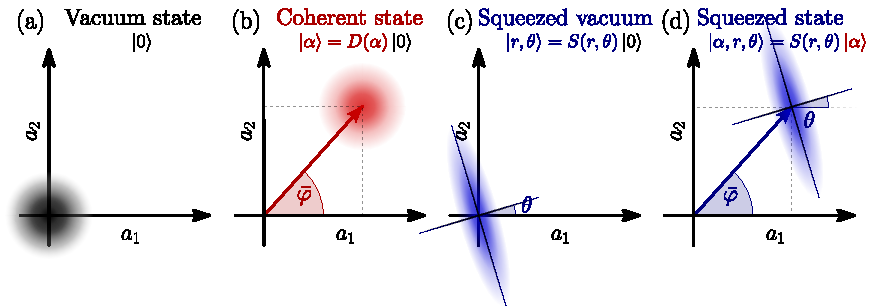
\includegraphics[width=\textwidth]{./chap2/fig/quantum_states.pdf}
\caption{Phase-space representations of quantum states and transformations.
(a) Wigner function of the vacuum state: a circular Gaussian centered at the origin, representing equal quantum fluctuations in both quadratures $a_1$ and $a_2$.
(b) Wigner function of a coherent state: a displaced circular Gaussian, showing a shift in phase space along an angle $\varphi$ with unchanged, isotropic noise.
(c) Wigner function of a squeezed vacuum state: an elliptical Gaussian centered at the origin, with reduced noise along a rotated quadrature $X_\theta$ and increased noise in the orthogonal direction.
(d) Wigner function of a displaced squeezed state: an ellipse shifted away from the origin, combining anisotropic fluctuations and a nonzero mean amplitude. The displacement angle $\varphi$ and squeezing angle $\theta$ are independent.} 
\end{figure}


\subsection*{Squeezed States:}

Squeezed states $|\alpha, r, \theta\rangle $ are quantum gaussian states of light in which the noise (variance) of one quadrature is reduced below the vacuum level, at the expense of increased noise in the conjugate quadrature. The single-mode squeezed vacuum state is defined as
\begin{align}
|0, r, \theta \rangle = \hat{S}(r, \theta) |0\rangle , \quad \hat{S}(\theta) = \exp\left[\frac{r}{2}(e^{-2 i\theta} \hat{a}^2 - e^{-2 i\theta} \hat{a}^{\dagger 2})\right]
\end{align}
where $r$ is the squeezing parameter (strength) and $\theta$ is the squeezing angle i.e. the angle along which one quadrature is reduced below vacuum level. The most general Gaussian state is the displaced squeezed state, obtained by applying both the squeezing operator $\hat{S}(r, \theta)$ and the displacement operator $\hat{D}(\alpha)$ to the vacuum:
\begin{equation}
|\alpha, r, \theta\rangle = \hat{S}(r, \theta)\hat{D}(\alpha)|0\rangle
\end{equation}
where $\hat{D}(\alpha)$ displaces the state in phase space by the complex amplitude $\alpha$, defined similarly to the coherent state. \\

\noindent \textbf{Note:}  The displacement and squeezing operators do not commute, i.e. $\hat{D}(\alpha)\hat{S}(r, \theta) \neq \hat{S}(r, \theta)\hat{D}(\alpha)$. However, both orderings correspond to experimentally valid procedures: one can either squeeze the vacuum and then displace (e.g. by mixing with a coherent state ona beamsplitter), or squeeze a coherent state straight away (e.g. by seeding an optical parametric amplifier). The resulting state is always a displaced squeezed state, but the relative phase between displacement and squeezing may differ. \\

\noindent \textbf{Expectation values: }Using the usual quadratures defined in Eq~\eqref{II.2} and \eqref{II.4}, the expectation values in a displaced squeezed state are
\begin{equation}
\langle \mathbf{\hat{u}} \rangle
= 2
\begin{pmatrix}
\mathrm{Re}\,\alpha \\[2pt]
\mathrm{Im}\,\alpha
\end{pmatrix}, 
\qquad
\langle \mathbf{\hat{u}_\phi} \rangle
= 2
\begin{pmatrix}
\mathrm{Re}\!\left(\alpha e^{-i\phi}\right) \\[2pt]
\mathrm{Im}\!\left(\alpha e^{-i\phi}\right)
\end{pmatrix}.
\label{II.xx3}
\end{equation}
For a squeezed vacuum ($\alpha=0$) all quadrature means vanish.
Choosing $\phi = \theta$, the fluctuations along the squeezing axis are
\begin{equation}
\langle \delta \hat a_\theta^2  \rangle = e^{-2r}, \qquad
\langle \delta \hat a_{\theta+\pi/2}^2 \rangle = e^{2r}, \qquad
\mathrm{Cov}(\hat a_\theta, \hat a_{\theta+\pi/2}) = 0,
\end{equation}
with uncertainty product $\Delta \hat a_\theta\, \Delta \hat a_{\theta+\pi/2} = 1$ saturating the Heisenberg bound.
The corresponding mean vector is
\begin{equation}
\langle \mathbf{\hat{u}_\theta} \rangle
= 2
\begin{pmatrix}
\mathrm{Re}(\alpha e^{-i\theta}) \\[2pt]
\mathrm{Im}(\alpha e^{-i\theta})
\end{pmatrix}.
\label{II.xx7}
\end{equation}

\begin{figure}
\centering
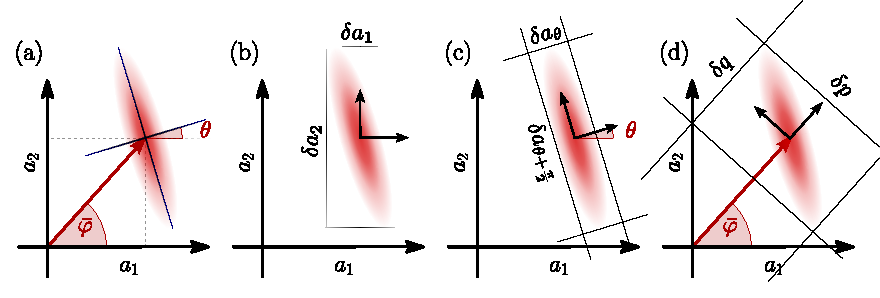
\includegraphics[width=\textwidth]{./chap2/fig/quantum_quadraturesBis.pdf}
\caption{Phase-space representations of quantum states and transformations.
(a) Wigner function of the vacuum state: a circular Gaussian centered at the origin, representing equal quantum fluctuations in both quadratures $X_1$ and $X_2$.
(b) Wigner function of a coherent state: a displaced circular Gaussian, showing a shift in phase space along an angle $\varphi$ with unchanged, isotropic noise.
(c) Wigner function of a squeezed vacuum state: an elliptical Gaussian centered at the origin, with reduced noise along a rotated quadrature $X_\theta$ and increased noise in the orthogonal direction.
(d) Wigner function of a displaced squeezed state: an ellipse shifted away from the origin, combining anisotropic fluctuations and a nonzero mean amplitude. The displacement angle $\varphi$ and squeezing angle $\theta$ are independent. \color{red} mistake on p and q  \color{black}}
\end{figure}

\noindent \textbf{Covariance matrix: }

Let $\psi \equiv \phi - \theta$ be the measurement angle $\phi$ relative to the squeezing axis $\theta$.  
For a displaced squeezed state, the covariance matrix is
\begin{equation}
\mathbf{V}_\phi = \mathbf R(\psi)
\begin{pmatrix}
e^{-2r} & 0 \\[2pt]
0 & e^{2r}
\end{pmatrix}
\mathbf R(\psi)^{T}.
\label{II.xx4}
\end{equation}
Expanding this explicitly gives

\begin{equation}
\mathbf{V}_\phi =
\begin{pmatrix}
\cosh 2r - \sinh 2r \cos 2\psi
& \sinh 2r \sin 2\psi \\[6pt]
\sinh 2r \sin 2\psi
& \cosh 2r - \sinh 2r \sin 2\psi
\end{pmatrix}.
\end{equation}
The covariance term is therefore
\begin{equation}
\mathrm{Cov}(\hat a_\phi, \hat a_{\phi+\pi/2})
= \sinh 2r \sin 2(\phi-\theta) ,
\label{II.xx6}
\end{equation}
which vanishes when $\sin 2(\phi-\theta) = 0$, i.e.\ $(\phi - \theta) \in \left\{ 0, \pi/2, \pi, \ldots \right\}$.
Along these principal axes of squeezing, $\mathbf{V}_\phi$ is diagonal. \\

\noindent \textbf{Amplitude and Phase squeezed states: }
Considering a displaced squeezed state, two special cases are of interest: the amplitude squeezed state where $\theta=\bar{\varphi}$ and the phase squeezed state where $\theta = \bar{\varphi}+\pi/2$. In the first case, the amplitude quadrature $\hat{p}$ is squeezed, while the phase quadrature $\hat{q}$ is anti-squeezed. In the second case, the phase quadrature is squeezed, while the amplitude quadrature is anti-squeezed. The covariance matrices for these states can be derived from Eq.~\eqref{II.xx4} by setting $\psi = 0$ or $\psi = \pi/2$, respectively. \\

\noindent \textbf{Photon number statistics: }

The mean and variance of the photon number operator $\hat N = \hat a^\dagger \hat a$ in a displaced squeezed state are
\begin{equation}
\langle \hat N \rangle = |\alpha|^2 + \sinh^2 r,
\qquad
\Delta N^2 = |\alpha|^2 \cosh 2r + \frac{1}{2} \sinh^2 2r.
\label{II.xx8}
\end{equation}
\color{red}
to rewrite
\color{black}
This shows that the squeezing operation increases the mean photon number of the coherent state by adding photons. Physically, this reflects the fact that generating squeezed light requires injecting energy into the system, so the squeezed vacuum contains correlated field excitations (photons) in even numbers. This is further seen by examining the photon-number distribution $P_n$: for a squeezed vacuum only even $n$ occur, while displacement progressively repopulates the odd $n$ and shifts weight to higher $n$, in agreement with the increase of $\langle \hat{N} \rangle$ and $\Delta N^2$ above.



\color{black}

\subsection{Sidebands and Quantum Noises}

\subsubsection{Modulation picture}
In realistic optical systems, the electromagnetic field is never perfectly monochromatic, nor isolated from its environment, nor static through time. Instead, it exhibits a finite spectral linewidth (stimulated emission, phase noise etc...), as well as non intentional/intentional modulations, all imprinted onto the carrier field. These effects cause the field amplitude and phase to evolve slowly compared to the optical frequency $\omega_0$. \\

As a result, the complex amplitude associated with each mode and described by the Schrodinger-picture annihilation operator $\hat{a}$, acquires an explicit time dependence beyond the standard fast-oscillating term $e^{-i\omega_0 t}$. It is often quoted as \textit{modulation} picture in the litterature. We then promote the field vector to 
\begin{equation}
\mathbf{\hat{a}}= \mathbf{\bar{a}} + \mathbf{\delta \hat{a}} \quad \rightarrow \quad
  \mathbf{\hat{a}}(t)=
 \mathbf{\bar{a}}(t) + \mathbf{\delta \hat{a}}(t)
\end{equation}
where the canonical commutation relations given in equation~\eqref{II.11} becomes:
\begin{equation}
  [\delta\mathbf{\hat{a}}(t), \delta \mathbf{\hat{a}}^{\dagger}(t')] = \mathbf{\sigma_z} \, \delta (t-t').
\end{equation}
and the covariance matrix of the ammplitude-phase quadratures turns to
\begin{equation}
\mathbf{V}(t, t') = \begin{pmatrix}
\langle \delta \hat{p}(t) \delta \hat{p}(t') \rangle &
\mathrm{Cov}(\hat{p}(t),\hat{q}(t')) \\[4pt]
\mathrm{Cov}(\hat{q}(t),\hat{p}(t'))  &
\langle \delta \hat{q}(t) \delta \hat{q}(t') \rangle 
\end{pmatrix} \delta(t-t')
\end{equation}
This time dependence allows us to track both slow classical modulations of the field $\mathbf{\bar{u}}(t)$ and the intrinsic quantum fluctuations $\mathbf{\delta \hat{u}(t)}$. Note this is equivalent to the interaction picture where the reference angular frequency would be $\omega_0$, but where we also consider dynamical processes way slower than this frequency. Additionally, we will always consider the limit of weak fluctuations, where the quantum noise can be treated perturbatively around the classical field i.e. 
\[
|\bar{\alpha}(t)| \gg \Delta \hat a_\theta(t)
\]
The resulting field operator can then be expressed as a 
\begin{equation}
\begin{aligned}
\hat{\mathbf{E}}(\mathbf{r}, t) 
=i  \mathcal{E}_0 \bigg[ & \left[ \alpha(t)\, \mathbf{f}(\mathbf{r})\, e^{-i \omega_0 t} 
- \alpha^*(t)\, \mathbf{f}^*(\mathbf{r})\, e^{i \omega_0 t} \right] \\
\quad +  &\left[ \delta \hat{a}(t)\, \mathbf{f}(\mathbf{r})\, e^{-i \omega_0 t}
- \delta \hat{a}^\dagger(t)\, \mathbf{f}^*(\mathbf{r})\, e^{i \omega_0 t} \right] \bigg]
\end{aligned}
\end{equation} 

\noindent \textbf{Amplitude Modulation (AM) :} Let the classical amplitude be modulated at $\Omega_{\text{mod}}$ in amplitude:
\begin{equation}
  \alpha(t) = \bar{\alpha} \left(1 + \epsilon_a \cos(\Omega_{\text{mod}} t)\right)
\end{equation}
with $\epsilon_a \ll 1$, the field amplitude modulation depth. While the DC term lives at frequency $\omega_0$, the modulation introduces sidebands at frequencies $\omega_0 \pm \Omega_{\text{mod}}$, seen by expanding the cosine:
\begin{equation}
  \alpha(t) = \bar{\alpha} \Big( 1 + \frac{\epsilon_a }{2}\, e^{i\Omega_{\text{mod}} t} + \frac{\epsilon_a }{2} \,  e^{-i\Omega_{\text{mod}} t} \Big)
\end{equation}


\noindent \textbf{Phase Modulation (PM) :} Now let the classical amplitude be modulated in phase at frequency $\Omega_{\mathrm{mod}}$:
\begin{equation}
\alpha(t) = \bar{\alpha} \, e^{i \epsilon_{\phi} \cos(\Omega_{\mathrm{mod}} t)}
\label{eq:PM_def}
\end{equation}
with $\epsilon_{\phi} \ll 1$ the field phase modulation depth. Expanding to first order in $\epsilon_{\phi}$ gives:
\begin{equation}
\alpha(t) \approx \bar{\alpha} \Big( 1 + \frac{i \epsilon_{\phi} }{2} \, e^{i\Omega_{\mathrm{mod}} t} + \frac{i \epsilon_{\phi} }{2} \, e^{-i\Omega_{\mathrm{mod}} t} \Big)
\label{eq:PM_expand}
\end{equation}
While the carrier term lives at frequency $\omega_0$, the modulation introduces sidebands at $\omega_0 \pm \Omega_{\mathrm{mod}}$, both shifted in phase by $\pi/2$ relative to the carrier.\\ 

In both cases, amplitude or phase modulations, the field contains a carrier at frequency $\omega$ and two sidebands at $\omega \pm \Omega$. Amplitude modulation results in sidebands that are in phase with the carrier, while phase modulation produces sidebands with a $\pm \pi/2$ phase shift relative to the carrier. We also note a general modulation process as :
\begin{equation}
\alpha(t) = \bar{\alpha} \left(1 + \varepsilon(t) \right)
\end{equation}
where $\varepsilon(t) \in \mathbb{C}$ is a modulation function that weakly modulates the complex amplitude in time, and that features information about the modulation frequency and depth. It then follows that the linearized amplitude-phase operators can be expressed as
\begin{equation}
\mathbf{\hat{\mathbf u}} _{\bar{\varphi}} (t) = 2|\bar{\alpha}| \begin{pmatrix}
  1 \\ 0 
\end{pmatrix} + 2|\bar{\alpha}|\begin{pmatrix}
  \mathrm{Re}\big(\varepsilon(t) \big) \\
  \mathrm{Im}\big(\varepsilon(t) \big)
\end{pmatrix}
+ \begin{pmatrix}
  \delta \hat{p}(t) \\
  \delta \hat{q}(t)
\end{pmatrix}
\end{equation}

\subsubsection{Fourier Domain}
To deal with noise spectra, we need to rewrite the various quadratures defined in the previous sections in the Fourier domain, where each frequency component is referred to as a \textit{sideband}.


The Fourier transform of the field vector is defined as
\begin{equation}
  \begin{split}
    \mathbf{\hat{a}}[\Omega] &=\int_{-\infty}^{+\infty}  dt \, e^{i\Omega t} \, \mathbf{\hat{a}}(t)\\
\mathbf{\hat{a}}(t) &= \frac{1}{2\pi}\int_{-\infty}^{+\infty}  d\Omega \, e^{-i\Omega t} \, \mathbf{\hat{a}}[\Omega]
  \end{split}
\end{equation}
where $\Omega \ll \omega_0$ is the sideband frequency relative to the so called \textit{carrier} frequency $\omega_0$. \color{red}  Add somthing on the true integral bound i.e. bandwidth B  \color{black}In this definition, a notable property is that the hermitian conjugate in the time domain translates to a frequency inversion in the Fourier domain:
\begin{equation}
   \Big[\hat{a}(t)\Big]^{\dagger} = \hat{a}^\dagger(t),  \quad
   \Big[\hat{a}[\Omega]\Big]^{\dagger}  = \hat{a}^\dagger[-\Omega].
\end{equation}
To lighten the notation we will use $\hat{a}^\dagger[\pm\Omega]=\hat{a}_\pm$. Carrying out the linearization in the Fourier domain, we have
\begin{equation}
      \mathbf{\hat{a}}[\Omega] =\begin{pmatrix} \bar{\alpha}_+ \\ \bar{\alpha}^*_- \end{pmatrix} + \begin{pmatrix} \delta\hat{a}_+ \\ \delta\hat{a}^\dagger_- \end{pmatrix} = \mathbf{\bar{a}}[\Omega]+ \mathbf{\delta \hat{a}}[\Omega]
\end{equation}
with the fluctuations commutator reading
\begin{equation}
  [\delta \mathbf{\hat{a}}[\Omega], \delta \mathbf{\hat{a}}[\Omega']^{\dagger}] = \mathbf{\sigma_z} \, \delta(\Omega + \Omega').
\end{equation}
The quadrature operators in the Fourier domain are then written as 
\begin{equation}
  \begin{split}
      \mathbf{\hat{u}_\phi}[\Omega] & = \mathbf{R}(\phi) \, \mathbf{\Gamma} \,\mathbf{\bar{a}}[\Omega] + \mathbf{R}(\phi) \, \mathbf{\Gamma} \, \mathbf{\delta \hat{a}}[\Omega] \\
      & = \underbrace{2|\bar{\alpha}| \begin{pmatrix}
  \cos(\bar{\varphi}-\phi) \\[2pt]
  \sin(\bar{\varphi}-\phi)
\end{pmatrix} \delta(\Omega)}_{\text{classical part}} +
\underbrace{\begin{pmatrix}
  \delta \hat{a}_\phi[\Omega] \\[2pt]
\delta \hat{a}_{\phi+\pi/2}[\Omega] \end{pmatrix}}_{\text{quantum fluctuations}}
  \end{split}
\end{equation}
such that the amplitude-phase quadrature vector reads
\begin{equation}
      \mathbf{\hat{u}_{\bar{\varphi}}}[\Omega]  = 2|\bar{\alpha}| \begin{pmatrix}
  1 \\[2pt]
  0
\end{pmatrix} \delta(\Omega) +
\begin{pmatrix}
  \delta \hat{p}[\Omega] \\[2pt]
\delta \hat{q}[\Omega]
\end{pmatrix}
\quad \text{with} \quad
  \begin{pmatrix}
  \delta \hat{p}[\Omega] \\[2pt]
\delta \hat{q}[\Omega]
\end{pmatrix} = \begin{pmatrix}
  \delta \hat{a}_+ + \delta \hat{a}^\dagger_-\\[2pt]
i\big(\delta \hat{a}^\dagger_- - \delta \hat{a}_+\big)  
\end{pmatrix}
\label{eq:2photons}
\end{equation}

This very way of writing the field quadratures is known as the \textit{two-photon} formalism, introduced by Caves and Schumaker~\cite{Caves1985,Caves1985a}. Here, we wrote down a vector, linearized form, useful to compute spectra numerically (see section ??). Throughout the litterature, the amplitude-phase two-photon quadratures are called differently, namely $(a_I, a_Q)$ (Caves and Schumaker), $(X_1, X_2)$ (Gerry and Knight), $(X, Y)$ (Bachor and Ralph) or $(x, p)$ (Weedbrook et al.). We chose the $p, q$ convention to perpetuate the convention used at LKB. \\

\noindent\textbf{Note: }
In the modulation picture, fluctuations in the time domain appear as symmetric sidebands at \(+\Omega\) and \(-\Omega\).
Any experimentally accessible, real signal arises from the interference of these two sidebands (quadratures in homodyne detection, intensity fluctuations, photocurrent spectra); equivalently, Hermiticity in time forces Fourier components to couple \(+\Omega\) with \(-\Omega\).
Packaging the field as the two-photon vector \(\big(\hat a[\Omega],\,\hat a^\dagger[-\Omega]\big)^{T}\) therefore groups exactly the two degrees of freedom that generate a single measurable fluctuation at frequency \(\Omega\). This makes correlations between the sidebands (which are the essence of frequency-dependent squeezing) explicit and ensures that quadrature spectra remain manifestly real. By contrast, the vector \(\big(\hat a[\Omega],\,\hat a^\dagger[\Omega]\big)^{T}\) is convenient for per-frequency photon-number or passive-scattering calculations, but it obscures the intrinsic pairing required to form real observables, forcing one to carry \(-\Omega\) separately.
For the noise-spectral analysis pursued here, the sideband-pair representation is thus the phenomenologically natural and algebraically minimal choice.


\subsubsection{Modulations in Fourier space}

Computing the Fourier transform for amplitude and phase modulations yields
\begin{equation}
  \begin{split}
    \varepsilon^{AM}(\Omega) & = \frac{\epsilon_a}{2} \Big(\delta(\Omega - \Omega_{\text{mod}}) +\delta(\Omega + \Omega_{\text{mod}}) \Big)\\
    \varepsilon^{PM}(\Omega) & = \frac{i\epsilon_\phi}{2} \Big(\delta(\Omega - \Omega_{\text{mod}}) + \delta(\Omega + \Omega_{\text{mod}})\Big)
  \end{split}
\end{equation}
And the quadrature operators of a modulated field can be expressed as
\begin{equation}
\mathbf{\hat{\mathbf u}} _{\bar{\varphi}} [\Omega] =2|\bar{\alpha}| \begin{pmatrix}
  1 \\ 0 
\end{pmatrix}\delta(\Omega) + 2|\bar{\alpha}|\begin{pmatrix}
  \mathrm{Re}\big(\varepsilon[\Omega] \big) \\
  \mathrm{Im}\big(\varepsilon[\Omega] \big)
\end{pmatrix}
+ \begin{pmatrix}
  \delta \hat{p}[\Omega] \\
  \delta \hat{q}[\Omega]
\end{pmatrix}
\end{equation}

\subsubsection{Vacuum fluctuations}
Considering a vacuum state or a coherent state, the expectation values of the quadrature fluctuations moments in the Fourier domain are
\begin{equation}
  \langle \delta \mathbf{\hat{u}_{\phi}}[\Omega] \rangle = \mathbf 0, \quad
\langle \delta \mathbf{\hat{\mathbf u}}_{\phi}[\Omega] \, \delta \mathbf{\hat{\mathbf u}}_{\phi}^{T}[\Omega'] \rangle = 2\pi \delta(\Omega + \Omega') \mathbf{1}
\end{equation}
\subsubsection{Noise Spectra}
In this work, we will be interested in the amplitude and phase noise spectra, defined as
\begin{equation}
  \mathbf{S}_{\bar{\varphi}}[\Omega] =   \frac{1}{2\pi} \int \delta \Omega^{'} \langle \delta \mathbf{\hat{u}}_{\bar{\varphi}}[\Omega]\, \delta \mathbf{\hat{u}}_{\bar{\varphi}}^{T}[\Omega'] \rangle =  \frac{1}{2\pi} \int \delta \Omega^{'} \begin{pmatrix}
  \langle \delta \hat{p}[\Omega]\,\delta \hat{p}[\Omega'] \rangle & \langle \delta \hat{p}[\Omega]\,\delta \hat{q}[\Omega'] \rangle \\[4pt]
  \langle \delta \hat{q}[\Omega]\,\delta \hat{p}[\Omega'] \rangle & \langle \delta \hat{q}[\Omega]\,\delta \hat{q}[\Omega'] \rangle
  \end{pmatrix}
\label{eq:Sa}
\end{equation}

In our way of writing it, we include all time dependent processes inside de fluctuation operators i.e. $\varepsilon(t)$ and $\delta \hat{p}(t)$, $\delta \hat{q}(t)$ in the case of quadrature operators, as all terms in $\delta (\Omega)$ contribute to the DC part of the spectrum. \\

We illustrate this by computing the spectra of a coherent field modulated in amplitude. The amplitude-phase quadrature fluctuation part reads
\begin{equation}
  \delta \mathbf{\hat{\mathbf u}}_{\bar{\varphi}}[\Omega] = |\bar{\alpha}|\epsilon_a \begin{pmatrix}
  \delta(\Omega - \Omega_{\text{mod}}) +\delta(\Omega + \Omega_{\text{mod}}) \\
  0 
\end{pmatrix}
+ \begin{pmatrix}
  \delta \hat{p}[\Omega] \\
  \delta \hat{q}[\Omega]
\end{pmatrix}
\end{equation}
such that its covariance matrix reads 
\begin{equation}
\mathbf{S}_{\bar{\varphi}}[\Omega] =  2|\bar{\alpha}|^{2}\epsilon_a^{2}
\Big[ \delta(\Omega - \Omega_{\mathrm{mod}})
     + \delta(\Omega + \Omega_{\mathrm{mod}}) \Big] \begin{pmatrix}
  1 & 0 \\
  0 & 0
     \end{pmatrix} + \mathbf{1}
\end{equation}
As seen in the above expression, the covariance matrix display a sum of dirac functions corresponding to a classical amplitude modulation of the field, as well as a flat vacuum noise across all frequencies.
\subsubsection{Linear Optical Systems}
As we will develop further in the next section, the output fields of various optical systems can be expressed in a general linear form as
\begin{equation}
\mathbf{\delta \hat{u}_{\mathrm{out}}}[\Omega]
=
\mathbf{T}[\Omega] \, \mathbf{\delta \hat{u}_{\mathrm{in}}}[\Omega]
+ \mathbf{L}[\Omega]  \mathbf{\delta \hat{u}_{\mathrm{vac}}}[\Omega].
\end{equation}
where $\mathbf{T}[\Omega]$ and $\mathbf{L}[\Omega]$ are $2\times 2$ transfer matrices. The input and vacuum fields are assumed to be in the vacuum state, as well as being uncorrelated such that 
\begin{equation}
  \begin{split}
    \langle \mathbf{\delta \hat{u}_{\mathrm{in}}}[\Omega]  \mathbf{\delta \hat{u}_{\mathrm{in}}}^{T}[\Omega'] \rangle & = 2\pi \delta(\Omega+\Omega')\mathbf{S}_{\mathrm{in}}[\Omega]  \\
    \langle \mathbf{\delta \hat{u}_{\mathrm{vac}}}[\Omega]  \mathbf{\delta \hat{u}_{\mathrm{vac}}}^{T}[\Omega'] \rangle &=  2\pi \delta(\Omega+\Omega')\mathbf{1}  \\
    \langle \mathbf{\delta \hat{u}_{\mathrm{in}}}[\Omega]  \mathbf{\delta \hat{u}_{\mathrm{vac}}}^{T}[\Omega'] \rangle &= \mathbf{0}
  \end{split}
\end{equation}
so one can write 
\begin{equation}
  \langle \mathbf{\delta \hat{u}_{\mathrm{out}}}[\Omega]  \mathbf{\delta \hat{u}_{\mathrm{out}}}^{T}[\Omega'] \rangle =2\pi \delta(\Omega+\Omega') \Big(\mathbf{T}[\Omega] \mathbf{S}_{\mathrm{in}}[\Omega] \mathbf{T}^{T}[\Omega'] + \mathbf{L}[\Omega] \mathbf{L}^{T}[\Omega']\Big).
\end{equation}
Computing the noise spectra is then straightforward : 
\begin{equation}
  \mathbf{S}_{\mathrm{out}}[\Omega] = \mathbf{T}[\Omega] \mathbf{S}_{\mathrm{in}}[\Omega] \mathbf{T}^{\dagger}[\Omega] + \mathbf{L}[\Omega] \mathbf{L}^{\dagger}[\Omega] 
\end{equation}
where $\mathbf{T}^{T}[-\Omega] = \mathbf{T}^{\dagger}[\Omega]$, $\mathbf{L}^{T}[-\Omega] = \mathbf{L}^{\dagger}[\Omega]$, and $\mathbf{S}_{\mathrm{vac}}[\Omega] = \mathbf{1}$ for vacuum inputs.\\
For an arbitrary quadrature angle $\phi$, one can simply rotate the transfer matrices as
\begin{equation}
  \mathbf{T}_\phi[\Omega] = \mathbf{R}(\phi) \, \mathbf{T}[\Omega] \, \mathbf{R}(-\phi), \quad
  \mathbf{L}_\phi[\Omega] = \mathbf{R}(\phi) \, \mathbf{L}[\Omega] \, \mathbf{R}(-\phi)
\end{equation}
such that
\begin{equation}
  \mathbf{S}_{\mathrm{out}, \phi}[\Omega] = \mathbf{T}_\phi[\Omega] \mathbf{S}_{\mathrm{in}, \phi}[\Omega] \mathbf{T}_\phi^{\dagger}[\Omega] + \mathbf{L}_\phi[\Omega] \mathbf{L}_\phi^{\dagger}[\Omega]
\end{equation}



\subsection{Quantum Sideband Diagram }

Starting with the simplest case : the vacuum/coherent state. 
\section{Cavities}
Optical cavities are at the heart of this work, as they are used to coherently enhance the light-matter interaction in various systems, and also to filter and manipulate quantum states of light. In this section, we review the basic properties of optical cavities, their resonance conditions, and we derive the covariance matrices of their output fields. 

\subsection{Cavity Geometries and Stability Conditions}
An optical cavity is a structure that \textit{traps} photons by means of reflection between two or more mirrors. They can be either standing wave cavities, where the light bounces back and forth between two mirrors, or traveling wave cavities, where the light circulates in a loop. In both cases, the cavity supports discrete resonant modes determined by its geometry and the boundary conditions imposed by the mirrors. The stability criteria of a specific cavity configuration is derived considering the round trip ABCD matrix of the cavity describing how the complex beam parameter $q(z)$ introduced in \eqref{II.1} transforms after one round trip. The stability condition then simply reads as $-1 < (A+D)/2 < 1$. In the case of planar - travelling wave cavities, one needs to consider both the tangential and sagittal planes, as these cavities are astigmatic. The stricter condition, generally the sagittal plane one, then defines the stability range of the cavity.\\

\begin{figure}
\centering
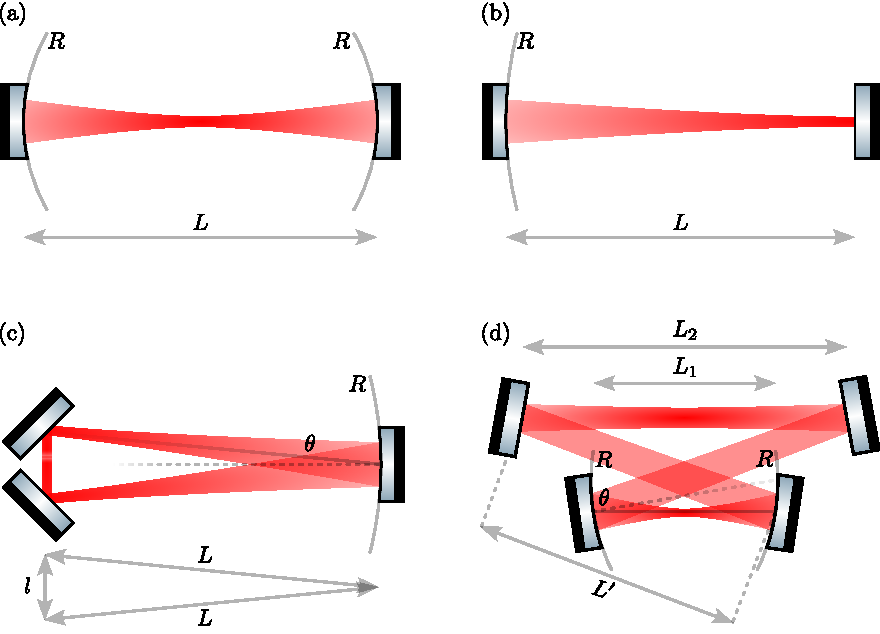
\includegraphics[width=\textwidth]{./chap2/fig/cavity_types.pdf}
\caption{Yes} 
\label{fig:cavity_types}
\end{figure}


\noindent \textbf{Linear standing wave cavities:} We first consider the two linear cavities used in this work, namely a confocal cavity (Fig \ref{fig:cavity_types}.(a)) with two identical concave mirrors, and a plano-concave cavity with one flat mirror and one concave mirror  (Fig \ref{fig:cavity_types}.(b)). Using the ABCD formalism for a confocal cavity of length $L$ formed by two identical mirrors of radii of curvature $R$, the stability condition reads
\begin{equation}
   \quad 0 < L < 2R
\end{equation}
For the plano-concave cavity, the stability condition reads
\begin{equation}
\quad 0 < L < R
\end{equation}

\noindent \textbf{Planar traveling wave cavities:} We now consider a triangular cavity formed by two concave mirrors of radius of curvature $R$ and one flat mirror  (Fig \ref{fig:cavity_types}.(c)). The stability condition reads
\begin{equation}
   \quad 0 < L_{rt} < 2R \cos(\theta)
\end{equation}
where $L_{rt} = 2L + l$ is the cavity round trip length, and $\theta$ is the angle of incidence of the beam onto the curved mirror. This condition is the sagittal one, and is more stringent than the tangential one.\\

Considering now a bow-tie cavity formed by two concave mirrors of radius of curvature $R$ and two flat mirrors  (Figure \ref{fig:cavity_types}.(d)), the full stability condition reads
\begin{equation}
  0 < \left( 1 - \frac{L_1 + 2L'}{R \cos\theta} \right) \left( 1 - \frac{L_2}{R \cos\theta} \right) < 1
\end{equation}
where $L_1$ is the distance between the two concave mirrors, $L_2$ the distance between the two flat mirrors, and $L'$ the distance between a concave and a flat mirror (assuming a symmetric cavity). A simple design rule guaranteeing stability is then to set $L_1 + 2L' < R \cos\theta$ and $L_2 < R \cos\theta$.\\


\subsection{Cavity Resonances}
If the cavity is stable, it will then feature a discrete set of resonant modes everytime the cavity length is an integer multiple of half the wavelength $\lambda/2$ (standing wave cavity) or the wavelength $\lambda$ (traveling wave cavity). In the frequency domain, modes are spaced by the free spectral range $\omega_{\mathrm{FSR}}$ of the cavity, defined as
\begin{equation}
  \omega_{\mathrm{FSR}} = \frac{\pi c}{L} \quad \text{(linear cavity)}, \quad \omega_{\mathrm{FSR}} = \frac{2 \pi c}{L_{rt}} \quad \text{(traveling wave cavity)}
\end{equation}
such that the resonant frequencies are given by
\begin{equation}
  \omega_m = m \, \omega_{\mathrm{FSR}}, \quad m \in \mathbb{N}
\end{equation}
and the cavity is on resonance when the input laser frequency $\omega_0$ matches one of the resonant frequencies $\omega_m$ i.e. $\omega_0 = \omega_m$. To achieve this, one can either tune the laser frequency or the cavity length. In our experiments, we use the second option by mounting one of the cavity mirrors on a piezoelectric actuator. Changing the cavity length $L$ by $\delta L$ shifts the resonant frequencies by
\begin{equation}
  \delta \omega_m = - m \, \frac{\pi c}{L^2} \, \delta L = - \frac{\omega_m}{L} \, \delta L
\end{equation}

\subsection{Mode-Matching}
A cavity also supports $TEM_{mn}$ transverse modes, each with a specific spatial profile and resonant frequency. The resonant frequencies of these transverse modes are shifted relative to the fundamental mode by an amount that depends on the cavity geometry and the mode indices $(m,n)$. Coupling an incoming beam into a stable optical cavity requires that the spatial mode of the beam matches that of the cavity. This means that the mode function of the incoming beam, assumed to be a TEM$_{00}$ Gaussian mode
 $f_{0}(\mathbf{r})$, must overlap with the cavity’s fundamental mode $f_{0}'(\mathbf{r})$. If the basis functions are not perfectly aligned, the incoming field can be expanded in the orthonormal basis of cavity modes as
\begin{equation}
    f_{0}(\mathbf{r}) = c_{0}\, f_{0}'(\mathbf{r}) + \sum_{m>0} c_{m}\, f_{m}'(\mathbf{r}),
\end{equation}
where the coefficients $c_{m}$ quantify the projection of the incident field onto the cavity eigenmodes. Only the component $c_{0} f_{0}'$ couples efficiently to the fundamental cavity mode due the mirror geometry, while any mismatch excites higher-order transverse modes $f_{m}'$. The mode-matching procedure therefore consists in maximizing the overlap integral
\begin{equation}
    \eta = \left| \int d^{3}\mathbf{r}\, f_{0}^{*}(\mathbf{r})\, f_{0}'(\mathbf{r}) \right|^{2},
\end{equation}
which ensures that essentially all the incoming photons populate the desired cavity mode, while suppressing excitation of spurious modes. \\

regarding the resonant lengths for which a speci

\subsection{\textrm{Simple} Cavities}

We consider a single field cavity mode described by the annihilation operator \(\hat{a}\), interacting with several independent noise inputs. The system is governed by a Hamiltonian 
\begin{equation}
\hat{H} = - \hbar \Delta  \hat{a}^\dagger \hat{a} 
\end{equation}
 with  $\Delta\equiv\omega_0 - \omega_c$ the cavity detuning to the laser frequency, and each input introduces dissipation characterized by a decay rate \(\kappa_i = T_i/\tau\), with $T_i$ the power transmittivity of the mirror and $\tau=2L/c$ the roundtrip time of the cavity. This is we consider an input coupler (mirror) with decay rate $\kappa_1$ and an output coupler (mirror) with decay rate $\kappa_2$. The laser field is shone onto the cavity by the input coupler. 
 
 
 In the modulation picture, the dynamics of \(\hat{a}\) is given by the Quantum Langevin Equation (QLE):
%
\begin{equation}
\begin{split}
  \frac{d}{dt} \hat{a}(t) & = -\frac{i}{\hbar} [\hat{a}, \hat{H}] - \frac{\kappa}{2} \hat{a}(t) + \sqrt{\kappa_1} \, \hat{a}_{\mathrm{in}}(t)  + \sqrt{\kappa_2} \, \delta \hat{a}_{\mathrm{vac}}(t) + \sqrt{\kappa_0} \, \delta \hat{a}_{\mathrm{l}}(t) \\
  & = -\Big(\frac{\kappa}{2}-i\Delta\Big) \hat{a}(t) + \sqrt{\kappa_{\mathrm{1}}} \, \hat{a}_{\mathrm{in}}(t)  + \sqrt{\kappa_2} \, \delta \hat{a}_{\mathrm{vac}}(t)  + \sqrt{\kappa_0} \, \delta \hat{a}_{\mathrm{l}}(t) 
\label{eq:qle}
\end{split}
\end{equation}
where  \(\kappa = \kappa_0 + \kappa_1 + \kappa_2\) is the total decay rate, with $\kappa_0=\gamma/\tau$ and $ \delta \hat{a}_{\mathrm{l}}(t)$ the rate and fluctuation operator of additional losses. Here losses $\gamma$ have ppm units. Another key element to deriving both steady state behaviour as well as quadrature spectra is the input-output formula given by:
\begin{equation}
  \hat{a}_{\mathrm{r}} = \sqrt{\kappa_{1}}\hat{a} - \hat{a}_{\mathrm{in}} , \quad \hat{a}_{\mathrm{t}} = \sqrt{\kappa_{2}}\hat{a} - \delta \hat{a}_{\mathrm{vac}} 
\end{equation}
for both the reflected and transmitted field. In the input-output formula, the $\hat{a}_{\mathrm{in}}$ refers to the field incoming on the coupler considered, which are simple vacuum fluctuations on the output coupler since we don't shine the laser by this port.\\

As introduced in the previous subsection, one can split the annihilation operator in a mean field part $\alpha$ and a fluctuation part $\mathbf{\delta \hat{a}}(t)$ (vector form) such that this equation turns into two i.e. a scalar differential equation, and an operator differentail equation, that is:
\begin{equation}
\left\{
\begin{aligned}
0 &= -\Big(\dfrac{\kappa}{2}-i\Delta\Big)\,\bar{\alpha}
    + \sqrt{\kappa_1}\,\bar{\alpha}_{\mathrm{in}} \\
 \mathbf{\delta \dot{\hat{a}}}(t)&
  = -\begin{pmatrix}
        \kappa/2-i\Delta & 0 \\
        0 & \kappa/2+i\Delta
      \end{pmatrix}\!
      \delta\hat{\mathbf{a}}(t)
     + \sqrt{\kappa_1}\,\delta\hat{\mathbf{a}}_{\mathrm{in}}(t)
     + \sqrt{\kappa_2}\,\delta\hat{\mathbf{a}}_{\mathrm{vac}}(t)
     + \sqrt{\kappa_0}\,\delta\hat{\mathbf{a}}_{\mathrm{l}}(t)
\end{aligned}
\right.
\tag{II.62}
\end{equation}

\begin{figure}
\centering
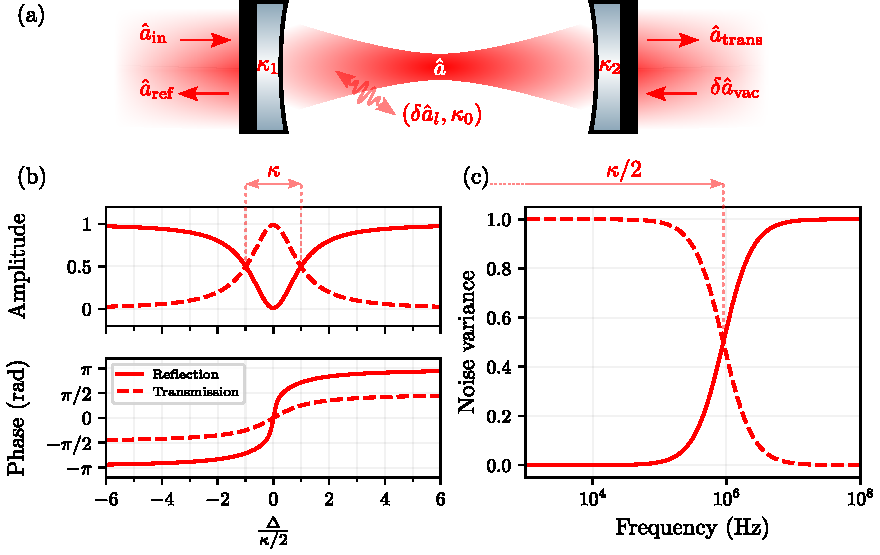
\includegraphics[width=\textwidth]{./chap2/fig/CavitySimple.pdf}
\caption{Yes} 
\label{fig:CavitySimple}
\end{figure}



\noindent \textbf{Mean field solution (Static case): }Taking the first scalar equation and expressing the mean intracavity field gives 
\begin{equation}
  \bar{\alpha} =  \frac{\sqrt{\kappa_1}}{\kappa/2-i\Delta}  \bar{\alpha}_{\mathrm{in}} 
\end{equation}
Patching it up with the input-output formula this gives 
\begin{equation}
  \bar{\alpha}_{\mathrm{r}} =  \Bigg( \frac{\kappa_1}{\kappa/2-i\Delta} - 1 \Bigg)  \bar{\alpha}_{\mathrm{in}}   \quad \quad \quad  \bar{\alpha}_{\mathrm{t}} =  \frac{\sqrt{\kappa_1 \kappa_2}}{\Big(\kappa/2-i\Delta\Big)} \bar{\alpha}_{\mathrm{in}}.
\end{equation}
The reflection and transmission coefficients are then
\begin{equation}
R(\Delta) = \left|\frac{\bar{\alpha}_{\mathrm{r}}}{\bar{\alpha}_{\mathrm{in}}}\right|^2
= \frac{\bigl(\kappa_1-\kappa/2\bigr)^2+\Delta^2}{\bigl(\kappa/2)^2+\Delta^2} \quad \quad
T(\Delta) = \left|\frac{\bar{\alpha}_{\mathrm{t}}}{\bar{\alpha}_{\mathrm{in}}}\right|^2
= \frac{\kappa_1\kappa_2}{\bigl(\kappa/2\bigr)^2+\Delta^2}.
\end{equation}
The cavity linewidth (FWHM) is then given by $\kappa$, as illustrated In Fig \ref{fig:CavitySimple}.(b). Plugging back the expression of $\kappa_i = T_i/\tau$ in the reflection coefficient, we have 
\begin{equation}
  R(\pm\infty) = 1  \qquad R(0) = \Bigg(\frac{T_1 - T_2 - \gamma}{T_1 + T_2 + \gamma}\Bigg)^2
\end{equation}
such that the relative depth of the resonance dip gives us information about the cavity losses and couplings. In particular, the resonance dip vanishes when $T_1 = T_2 + \gamma$, which is the so called \textit{impedance matching} condition: no light is reflected at resonance and all of it is transmitted or lost. \\ 

We also define the cavity finesse $\mathcal{F}$, which is a measure of the sharpness of the resonance peaks relative to its FSR, as
\begin{equation}
  \mathcal{F} = \frac{\omega_{\mathrm{FSR}}}{\kappa} = \frac{\pi c}{L \kappa} = \frac{2\pi}{T_1 + T_2 + \gamma}
\end{equation}
which also gives the average number of round trips a photon makes before escaping the cavity i.e. $\langle n_{rt} \rangle = \mathcal{F}/\pi$. For a given cavity length (so same FSR), the higher the finesse, the longer the photon lifetime in the cavity $\kappa^{-1}$. \\


\noindent \textbf{Mean field solution (Dynamical case): } \\
We now let the detuning vary linearly in time, and express it in units of cavity bandwidth as $\Delta(t)= \Delta_0 + v \frac{\kappa^2}{2}t$ where we defined $v$ as the sweep speed in units of cavity bandwidth per $\kappa^{-1}$. The intracavity field yields the standard differential equation
\begin{equation}
  \dot{\bar{\alpha}}(t)  + P(t)\bar{\alpha}(t) = Q(t)
\end{equation} 
with 
\begin{equation*}
  P(t) = \frac{\kappa}{2} - i\Big(\Delta_0 + v \frac{\kappa^2}{2}t\Big), \quad Q(t) = \sqrt{\kappa_1} \, \bar{\alpha}_{\mathrm{in}}(t)
\end{equation*}
ans is readily solved using an integrating factor such that,
\begin{equation}
  \bar{\alpha}(t) = e^{-\int_0^t P(t') dt'} \Bigg( \bar{\alpha}(0) + \int_0^t Q(t') e^{\int_0^{t'} P(t'') dt''} dt' \Bigg)
\end{equation}


This expression describes the transient response of the intracavity field as the detuning is swept through resonance. The reflected and transmitted fields can be obtained using the input-output relations, allowing one to analyze the dynamic behavior of the cavity under a time-varying detuning. This is particularly useful for understanding phenomena such as cavity ring-down and transient spectral features during rapid scans. \\


\noindent \textbf{Fluctuations solution: }To derive the covariance matrix we go to Fourier space such that 
\begin{equation}
     \mathbf{M}_\Delta \mathbf{\delta \hat{a}}[\Omega]  = \sqrt{\kappa_{\mathrm{1}}} \, \mathbf{\delta \hat{a}_{\mathrm{in}}}[\Omega]  + \sqrt{\kappa_2} \, \mathbf{\delta \hat{a}_{\mathrm{vac}}}[\Omega]   + \sqrt{\kappa_0} \, \mathbf{\delta \hat{a}_{\mathrm{l}}}[\Omega]   
\end{equation}
with 
\begin{equation*}
  \mathbf{M}_\Delta =\begin{pmatrix}
  \kappa/2-i(\Delta+\Omega) & 0 \\ 
  0 & \kappa/2+i(\Delta-\Omega)\\ 
  \end{pmatrix} 
\end{equation*}
The intracavity field fluctuations are then given by
\begin{equation}
  \mathbf{\delta \hat{a}}[\Omega]  = \mathbf{M}^{-1}_\Delta \Big( \sqrt{\kappa_1} \, \mathbf{\delta \hat{a}_{\mathrm{in}}}[\Omega] +  \sqrt{\kappa_2} \, \mathbf{\delta \hat{a}_{\mathrm{vac}}}[\Omega] +  \sqrt{\kappa_0} \, \mathbf{\delta \hat{a}_{\mathrm{l}}}[\Omega] \Big)
\end{equation}
and the reflected and transmitted fields read
\begin{equation}
  \begin{split}
  \mathbf{\delta \hat{a}_{\mathrm{r}}}[\Omega]  &= ( \kappa_1 \, \mathbf{M}^{-1}_\Delta - \mathbf{1} )\, \mathbf{\delta \hat{a}_{\mathrm{in}}}[\Omega] +  \sqrt{\kappa_1} \,\mathbf{M}^{-1}_\Delta (\sqrt{\kappa_2} \mathbf{\delta \hat{a}_{\mathrm{vac}}}[\Omega] + \sqrt{\kappa_0}  \mathbf{\delta \hat{a}_{\mathrm{l}}}[\Omega] ) \\
  \mathbf{\delta \hat{a}_{\mathrm{t}}}[\Omega] & =  \sqrt{\kappa_2} \,\mathbf{M}^{-1}_\Delta (\sqrt{\kappa_1} \mathbf{\delta \hat{a}_{\mathrm{in}}}[\Omega] + \sqrt{\kappa_0}  \mathbf{\delta \hat{a}_{\mathrm{l}}}[\Omega] ) +  (\kappa_2 \,\mathbf{M}^{-1}_\Delta - \mathbf{1}) \, \mathbf{\delta \hat{a}_{\mathrm{vac}}}[\Omega] 
  \end{split}
\end{equation}
Using $\delta \hat{\mathbf{a}} = \mathbf \Gamma^{-1} \delta \hat{\mathbf{u}}$ the reflected and transmitted quadratures read
\begin{equation}
  \begin{split}
  \mathbf{\delta \hat{u}_{\mathrm{r}}}[\Omega]  &= ( \kappa_1 \, \mathbf{\Gamma} \mathbf{M}^{-1}_\Delta \mathbf{\Gamma}^{-1}- \mathbf{1} )\, \mathbf{\delta \hat{u}_{\mathrm{in}}}[\Omega] +  \sqrt{\kappa_1} \,\mathbf{\Gamma}  \mathbf{M}^{-1}_\Delta \mathbf{\Gamma}^{-1} (\sqrt{\kappa_2} \mathbf{\delta \hat{u}_{\mathrm{vac}}}[\Omega] + \sqrt{\kappa_0}  \mathbf{\delta \hat{u}_{\mathrm{l}}}[\Omega] ) \\
  \mathbf{\delta \hat{u}_{\mathrm{t}}}[\Omega] & =  \sqrt{\kappa_2} \,\mathbf{\Gamma}  \mathbf{M}^{-1}_\Delta \mathbf{\Gamma}^{-1} (\sqrt{\kappa_1} \mathbf{\delta \hat{u}_{\mathrm{in}}}[\Omega] + \sqrt{\kappa_0}  \mathbf{\delta \hat{u}_{\mathrm{l}}}[\Omega] ) +  (\kappa_2 \,\mathbf{\Gamma}  \mathbf{M}^{-1}_\Delta \mathbf{\Gamma}^{-1}- \mathbf{1}) \, \mathbf{\delta \hat{u}_{\mathrm{vac}}}[\Omega] 
  \end{split}
\end{equation}
where the matrix product above reads 
\begin{equation*}
  \mathbf{\Gamma}  \mathbf{M}^{-1}_\Delta \mathbf{\Gamma}^{-1}
= \frac{1}{\left(\kappa/2-i\Omega\right)^{2}+\Delta^{2}}
\begin{pmatrix}
\kappa/2-i\Omega & \Delta \\[6pt]
-\Delta & \kappa/2-i\Omega
\end{pmatrix}.
\end{equation*}


The structure above is the engine behind frequency-dependent squeezing. On resonance, we have 
\begin{equation*}
\mathbf{M}_0^{-1} = \frac{1}{\kappa/2 - i\Omega} \mathbf{I} \quad \implies \quad  \mathbf{\Gamma} \mathbf{M}_0^{-1} \mathbf{\Gamma}^{-1} = \frac{1}{\kappa/2 - i\Omega} \mathbf{I}
\end{equation*}
causing symmetric sidebands around the carrier to be filtered identically both in amplitude and phase — so the quadrature along wich these sidebands are correlated (if considering squeezed correlations) remains the same at all frequencies. The moment the cavity is detuned, the $\mathbf{\Gamma}\mathbf{M}^{-1}_\Delta \mathbf{\Gamma}^{-1}$ off-diagonal terms asymmetrically mix the upper and lower sidebands; in the two-photon picture this is a frequency-dependent rotation and scaling of the $(p,q)$ basis. The amplitude (Lorentzian) part sets how strongly each sideband passes, while the phase accrued inside the cavity sets the rotation angle that now varies with $\Omega$. A broadband field with a single squeezing angle at the input is therefore converted into an output whose squeezing angle “twists” with frequency: near one band it can align with the phase quadrature, and at another it can align with the amplitude quadrature. This is exactly the mechanism exploited by filter cavities in precision interferometry: by choosing bandwidth, detuning, and coupling, one tailors the rotation profile to the target noise crossover. Practically, the attainable rotation and the preserved squeezing are limited by optical loss and mode mismatch, which inject uncorrelated vacuum and partially unwind the correlations the detuned cavity imprints on sidebands. \\



\noindent \textbf{Note: } On resonance ($\Delta=0$), the output quadratures can then be written as 
\begin{equation}
  \begin{split}
  \mathbf{\delta \hat{u}_{\mathrm{r}}}[\Omega]   &= \dfrac{\kappa_1-\kappa/2+i\Omega}{\kappa/2-i\Omega}  \,  \mathbf{\delta \hat{u}_{\mathrm{in}}}[\Omega]   +   \dfrac{\sqrt{\kappa_1 \kappa_2} }{\kappa/2-i\Omega}  \mathbf{\delta \hat{u}_{\mathrm{vac}}}[\Omega] + \dfrac{\sqrt{\kappa_1 \kappa_0} }{\kappa/2-i\Omega}  \mathbf{\delta \hat{u}_{\mathrm{l}}}[\Omega]  \\
  \mathbf{\delta \hat{u}_{\mathrm{t}}}[\Omega]   &= \, \dfrac{ \sqrt{\kappa_1 \kappa_2}}{\kappa/2-i\Omega}  \, \mathbf{\delta \hat{u}_{\mathrm{in}}}[\Omega]   +  \dfrac{\kappa_2-\kappa/2+i\Omega}{\kappa/2-i\Omega}   \mathbf{\delta \hat{u}_{\mathrm{vac}}}[\Omega]   + \dfrac{\sqrt{\kappa_2 \kappa_0} }{\kappa/2-i\Omega}  \mathbf{\delta \hat{u}_{\mathrm{l}}}[\Omega] 
  \end{split}
\end{equation}
If we consider the reflected quadratures noise spectra we see that 
\begin{equation}
   \mathbf{S}_{\mathrm{r}}[\Omega] =\frac{(\kappa_1-\kappa/2)^2+\Omega^2}{(\kappa/2)^2+\Omega^2}\,\mathbf{S}_{\mathrm{in}}[\Omega]+\frac{\kappa_1}{(\kappa/2)^2+\Omega^2}\,\Big(\kappa_2 \, \mathbf{1}+\kappa_0 \,\mathbf{1}\Big) 
\end{equation}
where the vacuum and loss covariance matrices are equal to \textbf{1}. As these two vacua sum up linearly, it is equivalent to consider a single vacuum with an effective decay rate $\kappa_2 + \kappa_0 \rightarrow \kappa_2$ to lighten the notation. We then absorb intrinsic losses into the output coupler, and consider only two ports: the input coupler with decay rate $\kappa_1$ and the output coupler with decay rate $\kappa_2$. We stress that this substitution is only valid when considering the \textbf{reflected} quadratures. When focusing on the transmitted quadratures, one can perform a similar redefinition with $\kappa_1$ i.e. $\kappa_1 + \kappa_0 \rightarrow \kappa_1$. \\


\noindent \textbf{Transfer matrices and Spectra:} Expressing the reflected and transmitted quadratures in matrix form yields
\begin{equation}
  \begin{split}
   \mathbf{\delta \hat{u}_{\mathrm{r}}}[\Omega] = \mathbf{T}_{\mathrm{r}}[\Omega]  \mathbf{\delta \hat{u}_{\mathrm{in}}}[\Omega] + \mathbf{L}_{\mathrm{r}}[\Omega]  \mathbf{\delta \hat{u}_{\mathrm{vac}}}[\Omega]
    \\
    \mathbf{\delta \hat{u}_{\mathrm{t}}}[\Omega] = \mathbf{T}_{\mathrm{t}}[\Omega]  \mathbf{\delta \hat{u}_{\mathrm{in}}}[\Omega] + \mathbf{L}_{\mathrm{t}}[\Omega]  \mathbf{\delta \hat{u}_{\mathrm{vac}}}[\Omega]
  \end{split}
\end{equation}
where the transfer matrices for the input and loss ports given by
\begin{equation*}
  \begin{split}
     \mathbf{T}_{\mathrm{r}}[\Omega]= \kappa_1 \, \mathbf{\Gamma} \mathbf{M}^{-1}_\Delta \mathbf{\Gamma}^{-1}- \mathbf{1}, \quad \mathbf{L}_{\mathrm{r}}[\Omega]=  \sqrt{\kappa_1 \kappa_2} \, \mathbf{\Gamma}  \mathbf{M}^{-1}_\Delta \mathbf{\Gamma}^{-1}\\
      \mathbf{T}_{\mathrm{t}}[\Omega]=   \sqrt{\kappa_1 \kappa_2} \, \mathbf{\Gamma}  \mathbf{M}^{-1}_\Delta \mathbf{\Gamma}^{-1}, \quad \mathbf{L}_{\mathrm{t}}[\Omega]= \kappa_2 \, \mathbf{\Gamma} \mathbf{M}^{-1}_\Delta \mathbf{\Gamma}^{-1}- \mathbf{1}
  \end{split}
\end{equation*}
such that the covariance matrices for the reflected and transmitted quadratures of a detuned cavity are given by
\begin{equation}
  \begin{split}
  \mathbf{S}_{\mathrm{r}}[\Omega] &= \mathbf{T}_{\mathrm{r}}[\Omega] \mathbf{S}_{\mathrm{in}}[\Omega] \mathbf{T}_{\mathrm{r}}^{\dagger}[\Omega] + \mathbf{L}_{\mathrm{r}}[\Omega] \mathbf{L}_{\mathrm{r}}^{\dagger}[\Omega] \\ \quad  \mathbf{S}_{\mathrm{t}}[\Omega] &= \mathbf{T}_{\mathrm{t}}[\Omega] \mathbf{S}_{\mathrm{in}}[\Omega] \mathbf{T}_{\mathrm{t}}^{\dagger}[\Omega] + \mathbf{L}_{\mathrm{t}}[\Omega] \mathbf{L}_{\mathrm{t}}^{\dagger}[\Omega]
  \end{split}
\end{equation}
Additionally, we define the one-photon reflection matrix of the input field by 
\begin{equation}
  \mathbf{r}_{\Delta}[\Omega] = \kappa_1 \, \mathbf{M}^{-1}_\Delta- \mathbf{1} = \begin{pmatrix}
    r_{\Delta}[\Omega] & 0 \\
    0 & r_{\Delta}^*[-\Omega]
  \end{pmatrix} \quad \text{with} \quad r_{\Delta}[\Omega] = \frac{\kappa_1 }{\kappa/2 - i(\Delta + \Omega)} - 1
\end{equation}
such that 
\begin{equation}
\mathbf{T}_{\mathrm{r}}[\Omega] = \mathbf{\Gamma} \, \mathbf{r}_{\Delta}[\Omega] \, \mathbf{\Gamma}^{-1} = \frac{1}{2}  \begin{pmatrix}
    r_{\Delta}[\Omega] + r_{\Delta}^*[-\Omega] & i(r_{\Delta}[\Omega] - r_{\Delta}^*[-\Omega]) \\
    -i(r_{\Delta}[\Omega] - r_{\Delta}^*[-\Omega]) & r_{\Delta}[\Omega] + r_{\Delta}^*[-\Omega]
  \end{pmatrix}
\end{equation}
and similarly for the one photon transmission matrix
\begin{equation}
  \mathbf{t}_{\Delta}[\Omega] = \sqrt{\kappa_1 \kappa_2} \, \mathbf{M}^{-1}_\Delta = \begin{pmatrix}
    t_{\Delta}[\Omega] & 0 \\
    0 & t_{\Delta}^*[-\Omega]
  \end{pmatrix} \quad \text{with} \quad t_{\Delta}[\Omega] = \frac{\sqrt{\kappa_1 \kappa_2}}{\kappa/2 - i(\Delta + \Omega)}
\end{equation}
such that
\begin{equation}
\mathbf{T}_{\mathrm{t}}[\Omega] = \mathbf{\Gamma} \, \mathbf{t}_{\Delta}[\Omega] \, \mathbf{\Gamma}^{-1} = \frac{1}{2}  \begin{pmatrix}
    t_{\Delta}[\Omega] + t_{\Delta}^*[-\Omega] & i(t_{\Delta}[\Omega] - t_{\Delta}^*[-\Omega]) \\
    -i(t_{\Delta}[\Omega] - t_{\Delta}^*[-\Omega]) & t_{\Delta}[\Omega] + t_{\Delta}^*[-\Omega]
  \end{pmatrix}
\end{equation}

\subsubsection{Example 1: Mode Cleaner }
Let us consider a configuration such that $\kappa_1 = \kappa_2 \approx \kappa/2$ where we assume negligible losses $\kappa_0 \ll \kappa_{1,2}$. It represents a cavity where the input and output mirror transmittivities are equal, and we set the laser resonant to the cavity ($\Delta=0$), such that the transmitted quadratures are written
\begin{equation}
  \mathbf{\delta \hat{u}_{\mathrm{t}}}[\Omega]  = \, \dfrac{ \kappa/2}{\kappa/2-i\Omega}  \, \mathbf{\delta \hat{u}_{\mathrm{in}}}[\Omega]   +  \dfrac{i\Omega}{\kappa/2-i\Omega}   \mathbf{\delta \hat{u}_{\mathrm{vac}}}[\Omega] .
\end{equation}
The resulting transmitted quadrature convariance matric is given by: 
\begin{equation}
  \mathbf{S}_{\mathrm{t}}[\Omega] =\frac{(\kappa/2)^2}{(\kappa/2)^2+\Omega^2} \, \mathbf{S}_{\mathrm{In}}[\Omega] +\frac{\Omega^2}{(\kappa/2)^2+\Omega^2}  \,  \mathbf{1}
\end{equation}
Now consider that the input fluctuations are above those of vacuum i.e. the input field features classical noise. We would then have $S_{pp}^{\rm in}> S_{pp}^{\rm vac}=1$ and $S_{qq}^{\rm in}> S_{qq}^{\rm vac}=1$. One can notice that the prefactor to the input noises is a Lorentzian function - a low pass filter. Hence, the noises of the input fields are low pass filtered by the cavity, while the vacuum fluctuations are high pass filtered at precisely the same cutoff $\kappa/2$. The mean field of the \textit{bright} coherent input is fully transmitted, but its super-vacuum fluctuations, potentially classically modulated, are filtered by the cavity. Taking a high finesse cavity such that the cutoff frequency is low, the transmitted field now features vacuum sidebands: it has been \textit{cleant} from classical noise. This is the principle of a \textit{mode cleaner} cavity, which is used in many precision experiments to provide a spectrally pure laser field, as well as a spatially filtered beam such that the transmitted beam is a pure $\mathrm{TEM}_{00}$.\\


\subsubsection{Example 2: Detuned single port cavity }
We now consider a lossless single port cavity with $\kappa_2 = 0$ and $\kappa_1 = \kappa$. The transfer matrix is expressed as 
\begin{equation}
  \mathbf{T}_{\mathrm{r}}[\Omega]=  \frac{1}{(\kappa/2 - i\Omega)^{2}+\Delta^{2}}
\begin{pmatrix}
     (\kappa/2)^2 - \Delta^2 + \Omega^2  & - \kappa \Delta  \\[6pt]
    + \kappa \Delta  & ( \kappa/2)^2 - \Delta^2 + \Omega^2 
\end{pmatrix}
\end{equation}

\begin{equation*}
\kappa \mathbf{\Gamma}  \mathbf{M}^{-1}_\Delta \mathbf{\Gamma}^{-1} - \mathbf{1} = \frac{1}{(\kappa/2 - i\Omega)^{2}+\Delta^{2}}
\begin{pmatrix}
      (\kappa/2)^2 - \Delta^2 + \Omega^2  & - \kappa \Delta  \\[6pt]
      + \kappa \Delta  & ( \kappa/2)^2 - \Delta^2 + \Omega^2
\end{pmatrix}
\end{equation*}
such that the covariance matrix is given by
\begin{equation}
  \mathbf{S}_{\mathrm{r}}[\Omega] = \begin{pmatrix}
    S_{pp}^{\mathrm{r}}[\Omega] & S_{pq}^{\mathrm{r}}[\Omega] \\[6pt]
    S_{qp}^{\mathrm{r}}[\Omega] & S_{qq}^{\mathrm{r}}[\Omega]
  \end{pmatrix}
\end{equation}
where we won't write the full expressions of the matrix elements for brevity. The key point is that the off-diagonal terms are non zero, meaning that the reflected quadratures are correlated. This is the frequency-dependent rotation mechanism described above.

This configuration is used in our experiment to measure the squeezing spectrum of the OPO, as the




\subsection{Non Linear Cavities}
We now turn to the description of optical cavities in which a $\chi^{(2)}$ medium is embedded within. This non linear medium can be used both for sum frequency generation, or difference frequency generation. The generic Hamiltonian describing a  degenerate $\chi^{(2)}$ parametric process is 
\begin{equation}
  H = \hbar \omega_p \hat{b}^{\dagger}\hat{b} + \hbar \omega_0 \hat{a}^\dagger \hat{a} + \frac{i\hbar\epsilon}{2}( \hat{b} \, \hat{a}^{\dagger2} - \hat{b}^\dagger \, \hat{a}^2)
\end{equation}
where we assumed perfect phase matching for simplicity, that is $\epsilon \in\mathbb{R}$. In our experiment wih squeezed light, we do use both as to first generate a pump field using a Second Harmonic Generation (SHG) scheme, then use the generated field to \textit{pump} a degenerate Optical Parametric Oscillator (OPO). The equations of motion of both fields are very similar in their structure, yet different in their phenomenology. Here we outline the main results and predictions for both. 
\begin{figure}
\centering
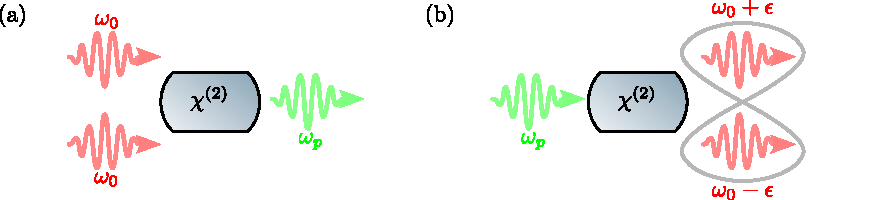
\includegraphics[width=\textwidth]{./chap2/fig/schema_SHG_OPO_2photons.pdf}
\caption{Yes} 
\end{figure}


\subsubsection{Second Harmonic Generation}

The SHG scheme consists in shining a laser field at frequency $\omega_0$ onto the cavity, and the non linear medium generates a field at frequency $\omega_p = 2\omega_0$, that is, two photons at $\omega_0$ described by operator $\hat{a}$, are converted into a single photon at $\omega_p$ described by operator $\hat{b}$. The input field is thus $\hat{a}_{\mathrm{in}}$ at $\omega_0$, while the input fields at $\omega_p$ are vacua $\hat{b}_{\mathrm{in}} = \delta {b}_{\mathrm{l}}= \delta \hat{b}_{\mathrm{vac}}$. We restrain the theoretical description to our experiment, where the end mirror reflectivity is $\sim 1$ for our generated green beam, as seen in the figure below $\kappa_{2,b}=0$. We will not derive the noise spectra for this scheme as they are not of interest in this work, displaying standard vacuum type fluctuations in both the pump and second harmonic field.
\begin{figure}[h]
\centering
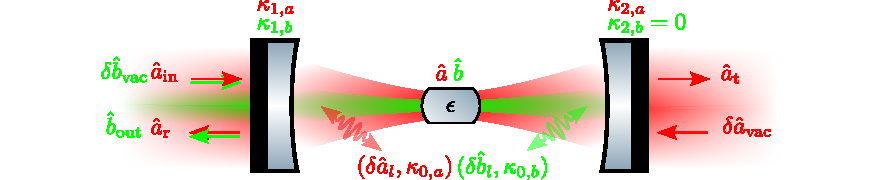
\includegraphics[width=\textwidth]{./chap2/fig/cavitySHG copy.pdf}
\caption{Yes} 
\end{figure}

We rather focus on the mean field solution. The scalar part of the QLE on resonance for both fields are given by 
 \begin{equation}
  \begin{split}
0 &= -\dfrac{\kappa_a}{2}\,\bar{\alpha} 
    + \epsilon\,\bar{\alpha}^{*}\,\bar{\beta} 
    + \sqrt{\kappa_{1,a}}\,\bar{\alpha}_{\mathrm{in}}, \\[6pt]
0 &= -\dfrac{\kappa_b}{2}\,\bar{\beta} 
    + \dfrac{\epsilon}{2}\,\bar{\alpha}^{2}.
  \end{split}
  \end{equation}
where subscript $a$ and $b$ refer to the $\omega_0$ and $\omega_p$ fields respectively. Solving for the $\bar{\beta}$ field and computing the output field $\bar{\beta}_{\mathrm{out}}$ from the input mirror using the input-output relations, yields an output intensity of 
\begin{align}
|\bar{\beta}_{\rm out}|^2
&= \frac{\kappa_{a}^{2}\kappa_{1,b}^{2}}{4\,\varepsilon^{2}}
\Bigg[
\Bigg(1+\frac{108\,\varepsilon^{2}\kappa_{1,a}}{\kappa_a^{3}\kappa_b}\,|\bar{\alpha}_{\rm in}|^{2}
\bigg(1+\sqrt{1+\frac{\kappa_a^{3}\kappa_b}{54\,\varepsilon^{2}\kappa_{1,a}\,|\bar{\alpha}_{\rm in}|^{2}}} \, \bigg)\Bigg)^{\!1/6} \nonumber \\[6pt]
&\qquad -
\Bigg(1+\frac{108\,\varepsilon^{2}\kappa_{1,a}}{\kappa_a^{3}\kappa_b}\,|\bar{\alpha}_{\rm in}|^{2}
\bigg(1+\sqrt{1+\frac{\kappa_a^{3}\kappa_b}{54\,\varepsilon^{2}\kappa_{1,a}\,|\bar{\alpha}_{\rm in}|^{2}}} \, \bigg)\Bigg)^{\!-1/6 \, }
\, \Bigg]^{\, 4}.
\end{align}
This cumbersome expression can be simplified in two limits. In the low input power limit, the output power scales quadratically with the input power, whereas at high powers it scales as $|\alpha_{\mathrm{in}}|^{4/3}$. \\

\noindent \textbf{Pseudo linear behaviour:} For intermediate powers, the output power scales almost linearly with the input power, which is precisely the regime in which we will operate. The crossover between these regimes is set by the non linear gain $\epsilon$ and the cavity decay rates $\kappa_{a,b}$. \\ 

\subsubsection{Optical Parametric Oscillation \& Amplification}
For this scheme, we consider a pump field with frequency $\omega_p = 2\omega_0$. A first key difference from the SHG scheme can be highlighted by the fact that we are now pumping at $2\omega_0$, such that pairs of entangled photons are generated at $\omega_0 + \epsilon$ and $\omega_0 - \epsilon$, with $\epsilon$ a sideband frequency allowed by the cavity bandwidth, hence conserving energy. 
\begin{figure}[h]
\centering
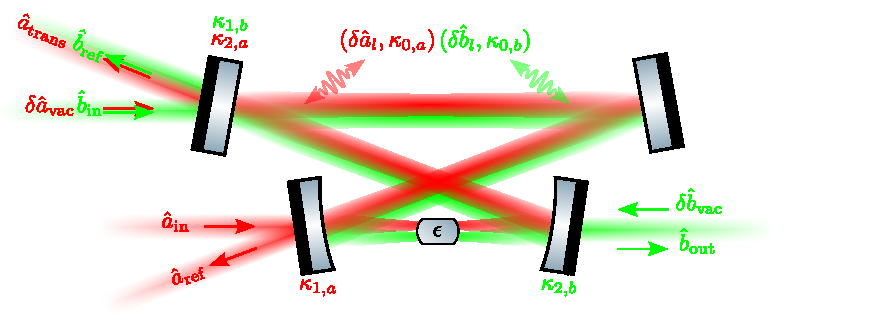
\includegraphics[width=\textwidth]{./chap2/fig/OPO2.pdf}
\caption{Yes} 
\end{figure}

We further consider the pump is not \textit{depleted}, such that we can change $\hat{b}$ to its mean field value $|\bar{\beta}|e^{i\bar{\varphi}_b}$, and we disregard the $\hat{b}$ fluctuations in the equations of motion for simplicity. A careful and complete derivations could also be carried out by keeping all terms in the equations of motion, but it is not serving our purpose here so we will these assumptions to lighten the notation. The total non linear gain is defined as $g = \epsilon |\bar\beta|$, and the QLEs for the steady state and fluctuation parts of the $\hat{a}$ field yields: 
 \begin{equation}
  \left\{
  \begin{split}
  0 &= -\Big(\frac{\kappa}{2}-i\Delta\Big) \bar{\alpha} +g e^{i\bar{\varphi}_b} \, \bar{\alpha}^* + \sqrt{\kappa_1} \, \bar{\alpha}_{\mathrm{in}} \\
  \mathbf{\delta \dot{\hat{a}}}(t)&= - \begin{pmatrix}
  \kappa/2-i\Delta & -g e^{i\bar{\varphi}_b}\\
   -g e^{-i\bar{\varphi}_b} & \kappa/2+i\Delta \\
  \end{pmatrix}  \mathbf{\delta \hat{a}}(t) + \sqrt{\kappa_{\mathrm{1}}} \, \mathbf{\delta \hat{a}_{\mathrm{in}}}(t)  + \sqrt{\kappa_2} \, \mathbf{\delta \hat{a}_{\mathrm{vac}}}(t)
  \end{split}
  \right.
\end{equation}
\noindent \textbf{Mean field solution (Static case): }Assuming a real input field $\bar{\alpha}_\textrm{in}=|\bar{\alpha}_\textrm{in}|$, the transmitted field is given by: 
\begin{equation}
   \bar{\alpha}_{\mathrm{t}} = \frac{\sqrt{\kappa_1\kappa_2}}{\kappa/2} \, \frac{1+i\dfrac{\Delta}{\kappa/2}+xe^{i\bar{\varphi}_b}}{1+\Big(\dfrac{\Delta}{\kappa/2}\Big)^2 - |x|^2}  |\bar{\alpha}_\textrm{in}|
\end{equation}
where we define the normalised pump parameter $x = 2g / \kappa \in\mathbb{R}$. This normalised pump parameter also equals the ratio of the pump field amplitude by the pump field threshold often written $B/B_{\mathrm{thr}}$. For a resonant cavity, the expression reduces to the well known parametric amplification/deamplification scheme 
\begin{equation}
   \bar{\alpha}_{\mathrm{t}} =  \frac{\sqrt{\kappa_1\kappa_2}}{\kappa/2}\frac{1+x e^{i\bar{\varphi}_b}}{1 - |x|^2} | \bar{\alpha}_\textrm{in} |
\end{equation}
in which the amplification or deamplification processes are set by the phase of the pump $\bar{\varphi}_b$. In the absence of a non linear medium $x=0$ we recover the standard cavity results shown above. The threshold is defined at $x=1$, where the rate of generation of entangled pairs exceeds the rate at which they leak from the cavity. In other words, $x$ is unity when the round trip gain equals the round trip losses. That's precisely the point where the no depletion approximation breaks down, as illustrated by the divergence seen in transmitted field at this very value (how could one obtained a diverging field from a pump field with a finite number of photons). We also notice two special cases, when $\bar\varphi_b=\{0,\pi\}$, coinciding with the amplification and the deamplification processes respectively. \\

\begin{figure}[h!]
\centering
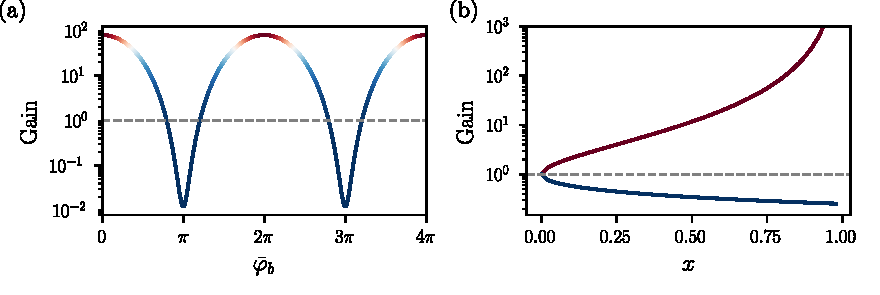
\includegraphics[width=\textwidth]{./chap2/fig/amp_deamp.pdf}
\caption{Yes} 
\end{figure}

\noindent \textbf{Fluctuations solution: } The general expression of the QLE in Fourier space is given by 
\begin{equation}
  \tilde{\mathbf{M}}_\Delta \,  \mathbf{\delta \hat{a}}[\Omega]  = \sqrt{\kappa_{\mathrm{1}}} \, \mathbf{\delta \hat{a}_{\mathrm{in}}}[\Omega]  + \sqrt{\kappa_2} \, \mathbf{\delta \hat{a}_{\mathrm{vac}}}[\Omega]
\end{equation}
with
\begin{equation*}
  \tilde{\mathbf{M}}_\Delta = \begin{pmatrix}
  \kappa/2-i(\Delta+\Omega) & -g e^{i\bar{\varphi}_b}\\
   -g e^{-i\bar{\varphi}_b} & \kappa/2+i(\Delta-\Omega) \\
  \end{pmatrix}
\end{equation*}
where we defined $\tilde{\mathbf{M}}_\Delta$ to not be confused with the matrix $\mathbf{M}_\Delta$ defined earlier for a simple cavity.
Note that a genuine \textit{frequency dependent} squeezing angle could be obtained by detuning the OPO cavity, but the frequency range over which the squeezing angle varies is limited by the cavity bandwidth, which is typically small compared to the frequency range of interest in our experiment. This phenomenon was realised experimentally few years ago \cite{Vahlbruch2006}, but is not the focus of our work. \\

In the context of our work, we will assume : 
\begin{itemize}
  \item the pump phase is locked to $\bar{\varphi}_b = \{0,\pi\}$ i.e. amplification or deamplification regime,  
  \item the cavity is resonant $\Delta=0$,
\end{itemize}
We further normalise all frequencies to the cavity bandwidth $\kappa/2$ such that $\Omega \rightarrow \Omega/(\kappa/2)$ and $g \rightarrow g/(\kappa/2) = x$, such that the off diagonal terms below can simply be written $\mp x$ factoring out the cavity bandwidth. We carry out the derivation for $\bar \varphi_b = 0$ (amplification) for simplicity, and the $\bar \varphi_b = \pi$ (deamplification) case is obtained by changing $x$ to $-x$ in the final expressions. The matrix QLE in Fourier space is written as
\begin{equation}
     \tilde{\mathbf{M}}_0 \,  \mathbf{\delta \hat{a}}[\Omega]  = \sqrt{\kappa_{\mathrm{1}}} \, \mathbf{\delta \hat{a}_{\mathrm{in}}}[\Omega]  + \sqrt{\kappa_2} \, \mathbf{\delta \hat{a}_{\mathrm{vac}}}[\Omega]  
\end{equation}
with 
\begin{equation*}
  \tilde{\mathbf{M}}_0 = \frac{\kappa}{2}\begin{pmatrix}
  1-i\dfrac{\Omega}{\kappa/2} & - x\\ 
  - x  & 1-i\dfrac{\Omega}{\kappa/2}\\ 
  \end{pmatrix} 
\end{equation*}

\noindent \textbf{Transfer matrices and Spectra: }
As before with a simple cavity, the transmitted quadratures at resonance are then 
\begin{equation}
\begin{split}
  \mathbf{\delta \hat{u}_{\mathrm{OPO}}}[\Omega] & =  \mathbf{T}_{\mathrm{OPO}}[\Omega] \mathbf{\delta \hat{u}_{\mathrm{in}}}[\Omega] +  \mathbf{L}_{\mathrm{OPO}}[\Omega] \, \mathbf{\delta \hat{u}_{\mathrm{vac}}}[\Omega] 
\end{split}
\end{equation}
where we defined the transfer matrices for the input and loss ports as
\begin{equation*}
  \mathbf{T}_{\mathrm{OPO}}[\Omega]=  \sqrt{\kappa_1 \kappa_2 } \,\mathbf{\Gamma}  \tilde{\mathbf{M}}^{-1}_0 \mathbf{\Gamma}^{-1}, \quad \mathbf{L}_{\mathrm{OPO}}[\Omega]=  \kappa_2 \,\mathbf{\Gamma}  \tilde{\mathbf{M}}^{-1}_0 \mathbf{\Gamma}^{-1}- \mathbf{1}....
\end{equation*}

After a bit of algebra, the covariance matrix of the transmitted field at $\bar \varphi_b = 0$ is then computed as
\begin{equation}
      \mathbf{S}^{0}_{\rm OPO}[\Omega] =\begin{pmatrix}
        1 + \dfrac{\kappa_2}{\kappa} \dfrac{4x}{(1- x)^2+ \Big(\dfrac{\Omega}{\kappa/2}\Big)^2} & 0 \\[10pt]
        0 & 1 - \dfrac{\kappa_2}{\kappa} \dfrac{4x}{(1+ x)^2+ \Big(\dfrac{\Omega}{\kappa/2}\Big)^2} 
      \end{pmatrix}
      \label{eq:II85}
\end{equation}




On a side note, when deriving the noise spectra for the intracavity field, the maximum amount of squeezing is limited to 3dB, while the transmitted field can feature arbitrarily high squeezing levels. This is interpreted as additional correlations between vacuum fluctuations being reflected at the output port of the OPO and the squeezed field leaking from this very same output port, allowing for strong squeezing. \\

\noindent \textbf{The perfect squeezer: } Starting from \eqref{eq:II85}, in the idealized limit of perfect escape efficiency ($\eta_{\rm esc}=1$) and for analysis frequencies much smaller than the cavity bandwidth ($\Omega/\kappa \to 0$), the expression simplifies to

\begin{equation}
      \mathbf{S}^{0}_{\rm OPO}[\Omega] =\begin{pmatrix}
         \dfrac{(1 + x)^2}{(1 - x)^2} & 0 \\[10pt]
        0 & \dfrac{(1 - x)^2}{(1 + x)^2} 
      \end{pmatrix}
\end{equation}
Introducing the standard squeezing parameter $r$ through the relation $x=\tanh \frac{r}{2}$, one can rewrite the numerator and denominator as
\begin{equation*}
1 + \tanh \frac{r}{2} = \frac{e^{+ \frac{r}{2}}}{\cosh \frac{r}{2}}, 
\qquad
1 - \tanh \frac{r}{2} = \frac{e^{- \frac{r}{2}}}{\cosh \frac{r}{2}},
\end{equation*}
such that
\begin{equation*}
\frac{(1 \pm \tanh \frac{r}{2})^2}{(1 \mp \tanh \frac{r}{2})^2}
= \left(\frac{e^{\pm \frac{r}{2}}}{e^{\mp \frac{r}{2}}}\right)^2
= e^{\pm 2r}.
\end{equation*}
Thus when $\bar\varphi_b=\{0,\pi\}$, in the lossless, low-frequency limit the transmitted noise levels reduce to the well-known parametric result
\begin{equation}
      \mathbf{S}^0_{\rm OPO}[\Omega] =\begin{pmatrix}
         e^{+ 2r} & 0 \\
        0 & e^{- 2r} 
      \end{pmatrix} \quad \quad \text{and} \quad \quad
      \mathbf{S}^\pi_{\rm OPO}[\Omega] =\begin{pmatrix}
         e^{- 2r} & 0 \\
        0 & e^{+ 2r}
      \end{pmatrix}
      \label{eq:perfect_squeezer}
\end{equation}
where we can now establish that an amplified field ($\bar\varphi_b=0$) corresponds to a squeezed phase quadrature and an anti-squeezed amplitude quadrature, while a deamplified field ($\bar\varphi_b=\pi$) corresponds to a squeezed amplitude quadrature and an anti-squeezed phase quadrature. 
Later on, we will use this idealized expression to describe how squeezed light interacts with a mechanical resonator whose frequency is much smaller than the OPO bandwidth. \\

\noindent \textbf{Losses: } Squeezing is very sensitive to optical losses, which couple uncorrelated vacuum fluctuations into the squeezed field and degrade the squeezing level. The escape efficiency $\eta_{\rm esc}=\kappa_2/\kappa$ of the OPO cavity is one such loss mechanism, but there are many others in a real experiment: propagation losses, mode-mismatch, non-unity quantum efficiency of the photodetectors, etc. One can then distinguish between \textit{intracavity} losses, which are accounted for in the escape efficiency, and \textit{extracavity} losses, which we denote by $\eta_{\rm ext}$ and lump all other loss mechanisms into a single effective loss. The effect of these losses can be modeled as a beam-splitter mixing the squeezed field with vacuum fluctuations, such that the lossy covariance matrix is given by
\begin{equation}\mathbf{S}_{\rm det}[\Omega] = (1-\eta) \, \mathbf{S}^{\bar \varphi_b}_{\mathrm{OPO}}[\Omega] + \eta \, \mathbf{1}
  \label{II.xx3}
\end{equation}
This expression is actually true for any Gaussian state suffering from losses. \\ 
\begin{figure}[h!]
\centering
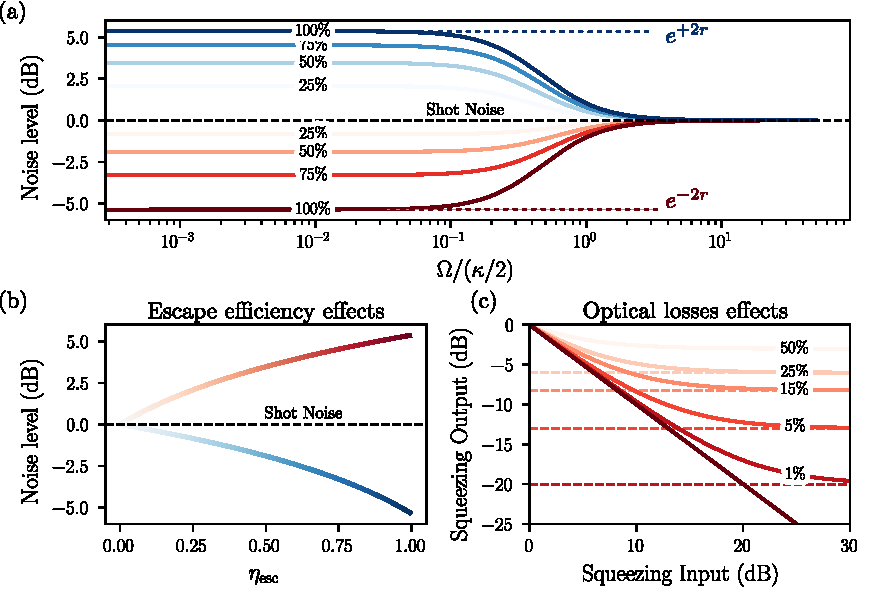
\includegraphics[width=\textwidth]{./chap2/fig/OPONoises.pdf}
\caption{Yes} 
\end{figure}


\noindent\textbf{Frequency dependence: } Similarly to what was seen earlier considering general quantum states, squeezing at an arbitrary angle $\theta$ can be obtained by rotating the covariance matrix. However, one can now make the squeezing angle frequency dependent
above as
\begin{equation}
\mathbf{S}^{\theta}_{\rm OPO}[\Omega] = \mathbf R(\theta[\Omega])
\mathbf{S}^0_{\rm OPO}[\Omega] 
\mathbf R^{\dagger}(\theta[\Omega]).
\label{II.xx4}
\end{equation}
where $\theta[]$
The $\mathbf{S}[\Omega]$ can either be the full cavity one, or the idealized one. As already mentionned, the mechanical frequencies of interest will be deep in the OPO bandwidth such that we will use the ideal squeezer expression \eqref{eq:perfect_squeezer} in addition with extrinsic losses \eqref{II.xx3}. The explicit of the covariance matrix at a frequency dependent angle is then
\begin{equation}
      \mathbf{S}^{\theta}_{\rm OPO}[\Omega] =\begin{pmatrix}
         \cosh 2r  - \sinh 2r \, \cos 2\theta[\Omega]  & -\sinh 2r \, \sin 2\theta[\Omega]  \\[10pt]
        -\sinh 2r \, \sin 2\theta[\Omega]  & \cosh 2r  + \sinh 2r \, \cos 2\theta[\Omega] 
      \end{pmatrix}
\end{equation}


\subsection{Optomechanical Cavities}
We now turn to standard optomechanical cavities. As in the simple FP case, we consider a cavity mode, in which we now allow one of the the coupler (traditionnaly the output coupler), to be itself a \textit{mechanical} harmonic oscillator with annihilation operator $\hat{c}$, effective mass $m$, angular frequency $\Omega_m$ and damping rate $\Gamma_m$. In canonical optomechanical systems the mechanics operators are usually denoted as $\hat b$ but in our case it would be redundant with the operators describing the pump field in non linear systems. The position can be expressed in terms of our bosonic operators as  $\hat{x}=x_0(\hat{c}+\hat{c}^{\dagger})$ with $x_0 = \sqrt{\hbar/(2m\Omega_m)}$ the resonator's zero point fluctuations. 

\begin{figure}[h!]
\centering
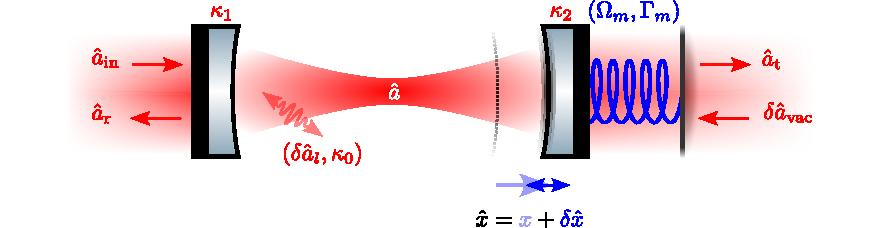
\includegraphics[width=\textwidth]{./chap2/fig/CavityOM.pdf}
\caption{Yes} 
\label{fig:cavity_types}
\end{figure}

\subsubsection{Mechanics \& Radiation Pressure Force }
The equation of motion of such an oscillator are given by 
\begin{equation}
  m \, \ddot{\hat x} = -m \, \Omega_m^2 \hat x - m \Gamma_m \dot{\hat x} + \hat F
\end{equation}
where $\hat F$ is the total force acting on the oscillator.
In Fourier space, we recover the standard linear response form
\begin{equation}
  \hat x [\Omega] = \chi[\Omega] \hat F[\Omega] \quad \text{with} \quad \chi[\Omega] = \frac{1}{m(\Omega_m^2 - \Omega^2 - i \Gamma_m \Omega)}
\end{equation}
where $\chi[\Omega]$ is the susceptibility linearly relating the position $\hat x [\Omega]$ to the external force $\hat F[\Omega]$. This susceptibility can also be written as 
\begin{equation}
  \chi[\Omega] = |\chi[\Omega]| e^{i \phi_m[\Omega]}
\end{equation}
with 
\begin{equation*}  
  \quad \text{with} \quad \phi_m[\Omega] = \arctan\Big(\frac{\Gamma_m \Omega}{\Omega_m^2 - \Omega^2}\Big) \quad \text{and} \quad |\chi[\Omega]| = \frac{1}{m\sqrt{(\Omega_m^2 - \Omega^2)^2 + (\Gamma_m \Omega)^2}}.
\end{equation*}


Similarly to the simple Fabry-Perot cavity (being a driven damped harmonic oscillator too), we can define the analog of the Finesse, namely the quality factor, defined as 
\begin{equation}
  Q = \frac{\Omega_m}{\Gamma_m}
\end{equation}
which is the number of oscillations before the resonator's energy is damped by a factor $1/e$. On resonance, the susceptibility is purely imaginary and reads $\chi[\Omega_m] = -i Q/(m \Omega_m^2)$. 

As before, the position is also linearized considering small quantum fluctuations compared to its mean value, such that we write $\hat{x}= x + \delta \hat{x}$. Importantly, the total position fluctuation $\delta \hat{x} = \Sigma \delta \hat{x}_i$ is the sum of individual fluctuations that can arise from various sources, such as a the zero point fluctuations, thermal fluctuations or radiation pressure induced fluctuations. In the following we will only consider a radiation pressure induced fluctuations $\delta \hat{x}_{\mathrm{RPN}}$, such that $\delta \hat{x} =  \delta \hat{x}_{\mathrm{RPN}}$. 

Due to the continuous yet discrete photon \textit{hits} at a rate exceeding the resonator frequency, the resonator \textit{feels} an effective force. This radiation pressure force is expressed as 
\begin{equation}
  \hat F = 2 \frac{\hbar k_L}{\tau_c}\hat{a}^\dagger \hat{a} = 2 \frac{\hbar k_L}{\tau_c} \, |\bar{\alpha}|^2 +2 \frac{\hbar k_L}{\tau_c} \, |\bar \alpha| \, \delta \hat{p} + \mathcal{O}(\delta \hat{a}^\dagger \delta \hat{a})
\label{eq:Frad}
\end{equation}
where $k_L = 2\pi / \lambda$ is the laser wavevector, and $\tau_c=2L/c$ is the cavity round-trip time, and we neglect second order terms. This force then features a static component shifting the resonator away from its equilibrium position, that be the $x$ component, as well as a fluctuating component $\delta \hat F\propto \delta \hat{p}$ jittering the resonator around its mean displacement, that's $\delta \hat x_{\mathrm{RPN}}$. The position mean value and its fluctuations under radiation pressure can therefore be expressed to first order as 
\begin{equation}
  x = \frac{2\hbar k_L |\bar \alpha|^2}{\tau_c}  \,  \chi[0] \, , \quad \delta \hat x_{\mathrm{RPN}} [\Omega]= \frac{2\hbar k_L |\bar \alpha|}{\tau_c}  \,  \chi[\Omega] \,  \delta \hat{p}[\Omega]. \label{eq:dx}
\end{equation} 



\subsubsection{Optomechanical QLE}
Considering an optomechanical cavity of length $L$ at rest, such that the mean resonator position is initialy 0, the bare cavity free spectral range is given by $\omega_{\mathrm{FSR}}=\pi c /L$ and the cavity frequency $\omega_c = N \omega_{\mathrm{FSR}}$. Injecting light inside this cavity then shifts the mechanical resonator position as seen above, which in turn changes the cavity length $L \rightarrow L+x$, thus its frequency. Writing the Hamiltonian, we simply Taylor expand to first order in $\hat{x}$ the cavity frequency $\omega_c(\hat{x})=\omega_c + \hat x \, \partial \omega_c / \partial x$ such that we have: 
\begin{equation}
\hat{H} = - \hbar \Delta  \hat{a}^\dagger \hat{a} + \hbar \, G  \hat{x} \, \hat{a}^{\dagger} \hat{a} + \hbar \, \Omega_m \hat{c}^\dagger \hat{c}
\end{equation}
where $G=  \partial \omega_c / \partial x = - \omega_c/L$. One can also identify a useful identity by considering the radiation pressure force \eqref{eq:Frad} and the Hamiltonian above, such that
\begin{equation}
  \hat F_{\textrm{rad}} = - \frac{\partial \hat H}{\partial \hat x} = - \hbar G \hat{a}^\dagger \hat{a} \quad \Rightarrow \quad G = - 2 \frac{k_L}{\tau_c}
\end{equation}
consistent with our previous expression of $G$ such that we rewrite the position fluctuation as $\delta \hat x_{\mathrm{tot}} [\Omega]= - \hbar G |\bar \alpha| \chi[\Omega]\, \delta\hat p[\Omega]$. 
Plugging in the QLE and ignoring vacuum and loss fluctuations for notational simplicity, the field's equation are written as 
\begin{equation}
  \left\{
  \begin{split}
  0 &= -\Big(\frac{\kappa}{2}-i\bar\Delta\Big) \bar{\alpha} + \sqrt{\kappa_1} \, |\bar{\alpha}_{\mathrm{in}}| \\
  \mathbf{\delta \dot{\hat{a}}}(t)&= - \begin{pmatrix}
  \kappa/2-i\bar\Delta & 0 \\ 
   0 &\kappa/2+i\bar\Delta \\ 
  \end{pmatrix}  \mathbf{\delta \hat{a}}(t) + iG\bar{\alpha}\delta \hat{x} \begin{pmatrix} +1 \\ -1\end{pmatrix}  +  \sqrt{\kappa_{\mathrm{1}}} \, \mathbf{\delta \hat{a}_{\mathrm{in}}}(t)  + \sqrt{\kappa_2} \, \mathbf{\delta \hat{a}_{\mathrm{vac}}}(t) 
  \end{split}
  \right.
\end{equation}
where we introduced the radiation pressure induced detuning $\bar\Delta = \Delta - G x$ - that is, the mean resonator displacement shifts the cavity frequency, hence the detuning - and where we assume the input field to be real. 

This so called \textit{dispersive} coupling, where the cavity frequency $\omega_c(x)$ depends linearly on the resonator's position to firs order, is the hallmark of the optomechanical interaction. In the canonical model, the cavity linewidth $\kappa$ do not depend on the resonator's position. \\

\noindent \textbf{Mean field solution \& Bistability:}
Writing the mean intracavity amplitude by keeping the \textit{unperturbed} detuning $\Delta$ for clarity and substituting for the static displacement $x$, we get
\begin{equation}
  \bar{\alpha} = \frac{\sqrt{\kappa_1}}{ \kappa/2 - i \Big( \Delta - \dfrac{\hbar G^2  |\bar{\alpha}|^2}{m_{\text{eff}} \Omega_m^2 } \Big)} |\bar{\alpha}_{\text{in}}|
\end{equation}
where the $|\bar{\alpha}|^2$ dependence in disguise in the mean mechanical displacement is the root of the bistable behaviour of optomechanical cavities. We show the induced hysteresis in figure ... 

For moderate injected powers, this is the standard intracavity field formula where we simply relabel $\Delta - Gx \rightarrow \Delta$ to lighten the notation. When resonant, the intracavity field does not pick up any phase and is real i.e. $\bar{\alpha} = |\bar{\alpha}| = 2\sqrt{\kappa_1}/\kappa \, |\bar{\alpha}_{\mathrm{in}}|$. 

Optomechanical cavities do display optical ringdowns too, as detailed in the cavity subpart above, but this is a purely optical phenomenon: the mechanics plays no role in the optical ringdwon (to first order?). \\


\noindent \textbf{Fluctuations solution:} As previously, going to Fourier space now yields 
\begin{equation}
     \mathbf{M}_{\bar\Delta} \mathbf{\delta \hat{a}}[\Omega]  = i \,  G \bar{\alpha}_{\mathrm{}} \delta \hat{x}[\Omega]   \begin{pmatrix} +1 \\ -1\end{pmatrix}  +\sqrt{\kappa_{\mathrm{1}}} \, \mathbf{\delta \hat{a}_{\mathrm{in}}}[\Omega]  + \sqrt{\kappa_2} \, \mathbf{\delta \hat{a}_{\mathrm{vac}}}[\Omega] 
\end{equation}
where we injected the mean field solution \eqref{eq:alpha} in our equations assuming moderate input power to ignore bistable behaviour. We focus on the resonant case to derive our noise spectra, such that $\mathbf{M}_0 = (\kappa/2 - i\Omega) \mathbf{I}$  and the intracavity quadratures are
\begin{equation}
  \mathbf{\delta \hat{u}}[\Omega] =  \frac{2G|\bar \alpha|}{\kappa/2 - i\Omega}\delta \hat{x}[\Omega] \begin{pmatrix} 0\\ 1\end{pmatrix}  +\frac{\sqrt{\kappa_{\mathrm{1}}}}{\kappa/2 - i\Omega} \, \mathbf{\delta \hat{u}_{\mathrm{in}}}[\Omega]  +\frac{\sqrt{\kappa_{\mathrm{2}}}}{\kappa/2 - i\Omega} \, \mathbf{\delta \hat{u}_{\mathrm{vac}}}[\Omega]  
\end{equation}
Writing explicitely our amplitude-phase quadratures then gives 
\begin{equation}
  \begin{split}
    \delta \hat{p}[\Omega] &= \frac{\sqrt{\kappa_{\mathrm{1}}}}{\kappa/2 - i\Omega} \, \delta \hat{p}_{\mathrm{in}}[\Omega] + \frac{\sqrt{\kappa_{\mathrm{2}}}}{\kappa/2 - i\Omega} \, \delta \hat{p}_{\mathrm{vac}}[\Omega] \\
    \delta \hat{q}[\Omega] &=  \frac{2G|\bar \alpha|}{\kappa/2 - i\Omega}\delta \hat{x}[\Omega]  +\frac{\sqrt{\kappa_{\mathrm{1}}}}{\kappa/2 - i\Omega} \, \delta \hat{q}_{\mathrm{in}}[\Omega]  + \frac{\sqrt{\kappa_{\mathrm{2}}}}{\kappa/2 - i\Omega} \, \delta \hat{q}_{\mathrm{vac}}[\Omega] 
  \end{split}
   \label{eq:intra_quad}
\end{equation}
This expression highlights the fact that only the phase is affected by the resonator position fluctuations. Physically, this can be understood by considering first that a fluctuating field amplitude leads to a fluctuating radiation pressure force, which in turn \textit{shakes} the mechanical resonator, which changes the phase of the field reflected. The reciprocal process does not happen: a fluctuating phase does not lead to a fluctuating radiation pressure force, hence the output amplitude fluctuations are unaffected by the mechanics. Importantly, considering the field reflected off the cavity we define the displacement to phase fluctuation transduction as
\begin{equation}
  \frac{\delta \hat{q}_x[\Omega]}{\delta \hat{x}[\Omega]} =  \frac{2\sqrt{\kappa_1}G|\bar \alpha|}{\kappa/2 - i\Omega} = \frac{\kappa_1}{\kappa} \dfrac{16 \mathcal{F}\sqrt{\bar{I}_{\rm in}}}{\lambda (1- i2\Omega/\kappa)}
\end{equation}
where we plugged in useful experimental parameters $\mathcal{F}$, $\lambda$ and $\bar I_{\rm in}$. The prefactor $\kappa_1/\kappa$ is the analog of the escape efficiency for optomechanical cavities, and is unity for single port cavities. We stress that the total phase fluctuations are the sum of various contributions, including the input phase fluctuations, the vacuum fluctuations entering from the loss port, and the position induced phase fluctuations, whether they arise from radiation pressure or other sources. This transduction factor will be used later to express the displacement sensitivity/spectra in terms of experimental parameters. \\


Plugging in the position fluctuations derived earlier (\eqref{eq:dx} and \eqref{eq:Frad}) in the intracavity phase fluctuations we get
\begin{equation}
  \begin{split}
\delta \hat{q}[\Omega] =  &\frac{\kappa_{\mathrm{1}}}{\kappa^2} \frac{8\hbar G^2|\bar \alpha_{\textrm{in}}|^2}{(\kappa/2 - i\Omega)^2}  \,  \chi[\Omega] \, \bigg( \sqrt{\kappa_1} \, \delta \hat{p}_{\mathrm{in}}[\Omega] + \sqrt{\kappa_2} \, \delta \hat{p}_{\mathrm{vac}}[\Omega] \bigg) \\ 
 & +\frac{1}{\kappa/2 - i\Omega} \, \bigg( \sqrt{\kappa_1} \, \delta \hat{q}_{\mathrm{in}}[\Omega] + \sqrt{\kappa_2} \, \delta \hat{q}_{\mathrm{vac}}[\Omega] \bigg) 
  \end{split}
\end{equation}
such that we can readily express the intracavity quadratures in matrix form as
\begin{equation}
\delta\mathbf{\hat{\mathbf u}} [\Omega]
=
\left(
\begin{array}{cc}
\dfrac{1}{\kappa/2 - i\Omega} & 0\\[6pt]
\dfrac{\mathcal{K}[\Omega]}{\kappa_1} & \dfrac{1}{\kappa/2 - i\Omega}
\end{array}-
\right)
\bigg( 
\sqrt{\kappa_1} \delta\mathbf{\hat{\mathbf u}} _{\mathrm{in}}[\Omega] +\;
\sqrt{\kappa_2} \delta\mathbf{\hat{\mathbf u}} _{\mathrm{vac}}[\Omega] \bigg)  \, .
\end{equation}
with
\begin{equation*}
  \mathcal{K}[\Omega] = \Bigl(\dfrac{\kappa_{\mathrm{1}}}{\kappa}\Bigr)^2 \dfrac{8\hbar G^2|\bar \alpha_{\textrm{in}}|^2}{(\kappa/2 - i\Omega)^2}  \,  \chi[\Omega] = \Bigl(\dfrac{\kappa_{\mathrm{1}}}{\kappa}\Bigr)^2 \dfrac{128 \hbar \mathcal{F}^2 \bar I_{\rm in}}{\lambda^2(1 - i2\Omega/\kappa)^2}  \,  \chi[\Omega]
\end{equation*}
We then obtain the reflected and transmitted quadrature fluctuations 
\begin{equation}
\begin{split}
\mathbf{\delta \hat{u}_{\mathrm{r}}}[\Omega] &= 
\mathbf{T}_{\mathrm{r}}[\Omega]
\delta\hat{\mathbf u}_{\mathrm{in}}[\Omega] + 
\mathbf{L}_{\mathrm{r}}[\Omega]
\delta\hat{\mathbf u}_{\mathrm{vac}}[\Omega] \, \\ 
\mathbf{\delta \hat{u}_{\mathrm{t}}}[\Omega] &= \mathbf{T}_{\mathrm{t}}[\Omega]  \delta\hat{\mathbf u}_{\mathrm{in}}[\Omega] +
\mathbf{L}_{\mathrm{t}}[\Omega]
\delta\hat{\mathbf u}_{\mathrm{vac}}[\Omega] \, .
\end{split}
\end{equation}
 where we defned the transfer matrices 
\begin{equation*}
  \begin{alignedat}{3}
     \mathbf{T}_{\mathrm{r}}[\Omega] &=\begin{pmatrix}
  \dfrac{\kappa_1}{\kappa/2-i\Omega}  -1  & 0 \\
  \mathcal{K}[\Omega]  &  \dfrac{\kappa_1}{\kappa/2-i\Omega}  -1 
\end{pmatrix}  \quad
 & \mathbf{L}_{\mathrm{r}}[\Omega] &= \begin{pmatrix}
   \dfrac{ \sqrt{\kappa_1 \kappa_2}}{\kappa/2-i\Omega}   & 0 \\
  \sqrt{\dfrac{\kappa_2}{\kappa_1}} \, \mathcal{K}[\Omega] &   \dfrac{ \sqrt{\kappa_1 \kappa_2}}{\kappa/2-i\Omega}  
\end{pmatrix} \\
        \mathbf{T}_{\mathrm{t}}[\Omega] &=  \begin{pmatrix}
   \dfrac{ \sqrt{\kappa_1 \kappa_2}}{\kappa/2-i\Omega}   & 0 \\
  \sqrt{\dfrac{\kappa_2}{\kappa_1}} \, \mathcal{K}[\Omega] &   \dfrac{ \sqrt{\kappa_1 \kappa_2}}{\kappa/2-i\Omega}  
\end{pmatrix}  \quad 
& \mathbf{L}_{\mathrm{t}}[\Omega]&= \begin{pmatrix}
  \dfrac{\kappa_2}{\kappa/2-i\Omega}  -1  & 0 \\
  \dfrac{\kappa_2}{\kappa_1}\mathcal{K}[\Omega]  &  \dfrac{\kappa_2}{\kappa/2-i\Omega}  -1 
\end{pmatrix} 
  \end{alignedat}
\end{equation*}


\noindent \textbf{Convergence to VIRGO/LIGO notation:} To sanity check this expression, we need to make sure we recover the standard expressions used in the LIGO/VIRGO community. This is we will assume the mechanical resonator is free, that is $\Omega_m \rightarrow 0$ and $\Gamma_m \rightarrow 0$. The susceptibility then reduces to $\chi[\Omega] = 1/ M \Omega^2$, and we will consider sideband frequencies $\Omega \ll \kappa/2$ such that all terms in $\Omega/(\kappa/2)$ can be neglected. We also consider a single port cavity such that $\kappa_1 = \kappa$ and $\kappa_2=0$. The reflected quadrature fluctuations then read
\begin{equation}
\mathbf{\delta \hat{u}_{\mathrm{r}}}[\Omega]
=
\begin{pmatrix}
  1   & 0 \\[12pt]
  \dfrac{32 \omega_0P_{\mathrm{in}}}{M L^2\kappa^2 \Omega^2}    &  1
\end{pmatrix}
\delta\hat{\mathbf u}_{\mathrm{in}}[\Omega].
\end{equation}
In GW papers, the pre factor will often be 8 (and not 32) as they use the cavity half width at half maximum rather than $\kappa$. We indeed recover the standard expression used in the GW community, which is a good sanity check of our derivation. We do stress however that this expression is only valid for a free mass, and that the full expression including the mechanical resonance is required to describe optomechanical cavities in general. \\


\noindent \textbf{Reflected spectra:} We can now compute the covariance matrix of the reflected quadratures, assuming vacuum fluctuations both at the input and at the loss port. We additionally consider a quasi single port cavity for simplicity $\kappa_1 \gg \kappa_2$, such that $\kappa_1\sim\kappa$, as well as the bad cavity limit $\Omega \ll \kappa/2$. The reflected covariance matrix is then given by
\begin{equation}
      \mathbf{S}_{\rm r}[\Omega] =\mathbf{T}_{\mathrm{r}}[\Omega] \mathbf{S}_{\text{in}}[\Omega] \mathbf{T}_{\mathrm{r}}^{\dagger}[\Omega]  = \begin{pmatrix}
        1 &  \mathcal{K}[\Omega]\\[6pt]
          \mathcal{K}^{*}[\Omega]& 1 +  |\mathcal{K}[\Omega]|^2
      \end{pmatrix}
\end{equation}
where the off-diagonal entries are complex conjugates of each other, ensuring the covariance matrix is Hermitian as required. The diagonal terms are the amplitude and phase noise spectra respectively, while the off-diagonal terms quantify correlations between amplitude and phase. The presence of these correlations is the hallmark of optomechanical/ponderomotive squeezing i.e. using the non linear response of the resonator to squeeze light. This effect is not seen nor seeked in our experiment, but is a very active field of research in the optomechanics community. \\

One now sees two essential components in the reflected phase spectrum. The first is the direct phase fluctuations, which is simply shot noise seen as $1$. The second is the back-action term $\propto |\mathcal{K}[\Omega]|^2$, which is the phase fluctuations induced by the resonator motion driven by radiation pressure fluctuations. 

